\documentclass[11pt,a4paper]{article}
\usepackage[margin=22mm,headheight=15pt]{geometry}
\usepackage[no-math]{fontspec}
\setmainfont{NotoSerifCJKsc-Regular.otf}[Path=assets/,BoldFont=NotoSerifCJKsc-Regular.otf,BoldFeatures={FakeBold=1.7},ItalicFont=NotoSerifCJKsc-Regular.otf,ItalicFeatures={FakeSlant=.12}]
\setsansfont{NotoSerifCJKsc-Regular.otf}[Path=assets/,BoldFont=NotoSerifCJKsc-Regular.otf,BoldFeatures={FakeBold=1.7}]
\setmonofont{DejaVu Sans Mono}[Scale=.85]
\XeTeXlinebreaklocale "zh"
\XeTeXlinebreakskip=0pt plus 1pt
\usepackage{amsmath,amssymb,mathtools,mathrsfs}
\usepackage{booktabs,longtable,array,calc}
\usepackage{graphicx,xcolor,fancyhdr,enumitem,needspace}
\usepackage{float}
\floatplacement{figure}{H}
\setkeys{Gin}{keepaspectratio}
\usepackage[unicode,breaklinks]{hyperref}
\hypersetup{colorlinks=true,linkcolor=black,urlcolor=blue!55!black,pdftitle={Research MAX-STRUCT：非线性 Maxwell 逆散射的结构发现},pdfauthor={Research MAX-STRUCT}}
\urlstyle{same}
\usepackage{xurl}
\setlength{\parindent}{0pt}
\setlength{\parskip}{5.5pt}
\setlength{\emergencystretch}{3em}
\widowpenalty=10000
\clubpenalty=10000
\displaywidowpenalty=10000
\linespread{1.18}
\setcounter{tocdepth}{2}
\setcounter{secnumdepth}{0}
\renewcommand{\contentsname}{目录}
\renewcommand{\figurename}{图}
\setlist{nosep,leftmargin=1.7em,topsep=4pt}
\newcommand{\tightlist}{\setlength{\itemsep}{0pt}\setlength{\parskip}{0pt}}
\providecommand{\pandocbounded}[1]{#1}
\providecommand{\real}{\operatorname{Re}}
\providecommand{\imag}{\operatorname{Im}}
\pagestyle{fancy}
\fancyhf{}
\fancyhead[L]{\small Research MAX-STRUCT}
\fancyhead[R]{\small 理论研究 · 2026-11-02}
\fancyfoot[C]{\small\thepage}
\renewcommand{\headrulewidth}{0.3pt}
\renewcommand{\arraystretch}{1.18}
\setlength{\LTpre}{7pt}
\setlength{\LTpost}{7pt}
\begin{document}
\begin{titlepage}
\vspace*{14mm}
{\Large 非线性 Maxwell 逆散射}\par
\vspace{8mm}
{\Huge\bfseries Research MAX-STRUCT}\par
\vspace{8mm}
{\LARGE 从物理约束、可观测商与全波谱序\par 发现新的数学问题}\par
\vspace{12mm}
{\large 超越局部反馈的结构研究与实验交接}\par
\vspace{14mm}
\begin{minipage}{.92\textwidth}
本报告的主张不是已经得到一个超过成熟 CIE-I 的反演器，而是确定三条具有独立物理内容、可以被严格证明或小实验推翻的研究主线：固定磁场约束空间；有限通道全波单调性；有限照明下的同场材料族。\par
报告明确区分经典结果、仓库既有成果、本轮条件推导、待证假说及实际运行的微型验证。
\end{minipage}
\vfill
{\large 研究日期：2026 年 11 月 2 日}\par
\vspace{3mm}
{\small 主仓库冻结版本：7317601b43b914525c21f09e5a60020552ea677b}\par
{\small A17 冻结版本：2ac81b989a2f13d62df9d5a7abd690a33c2189c7}\par
\vspace{7mm}
{\small 交付范围：中文理论报告、独立实验交接文件、推导与微型验证源文件。\par
本轮未启动新的大规模成像或参数扫掠；未修改、提交或推送研究仓库。}
\end{titlepage}
\tableofcontents
\clearpage
\hypertarget{ux7814ux7a76ux7ed3ux8bbaux4e0eux8bc1ux636eux8fb9ux754c}{%
\section{1.
研究结论与证据边界}\label{ux7814ux7a76ux7ed3ux8bbaux4e0eux8bc1ux636eux8fb9ux754c}}

\hypertarget{ux6700ux503cux5f97ux8865ux4e0aux7684ux7ed3ux6784ux662fux4ec0ux4e48}{%
\subsection{1.1
最值得补上的结构是什么}\label{ux6700ux503cux5f97ux8865ux4e0aux7684ux7ed3ux6784ux662fux4ec0ux4e48}}

\textbf{相对于当前以电流、材料反馈和双边响应为中心的研究路线，最值得补上的结构，是把``由
Maxwell 运动学决定的合法场空间''与``由材料决定的本构作用''分开。}
在三维矢量问题中，这不是一般的 Green 矩阵预分解：无自由电荷、源外 ROI
内的电场满足材料相关的
\(\nabla\cdot(\varepsilon E)=0\)，而已知磁导率时磁场满足固定的
\(\nabla\cdot(\mu H)=0\)。它提示一种更简单的状态选择，也直接联系到逆介电系数的算子序、内部激发秩和有限照明的不可辨识性。

本报告推荐三条竞争的主线，不要求把它们合成一个求解器。

\begin{enumerate}
\def\labelenumi{\arabic{enumi}.}
\tightlist
\item
  \textbf{固定磁场空间与材料 Hodge 场族。}
  先问磁场是否在能控制旋度、物理缺陷及观测误差的范数下，比传统电流
  Fourier
  空间更容易表示。若答案肯定，采用标准磁场形式就可能比增加反馈模块更简单。磁场形式及
  Hodge/shorted operator
  本身均是经典工具，创新必须落在新的统一逼近结论或同成本的逆散射能力上。
\item
  \textbf{有限通道的全波单调性排除。}
  全波数据不只给局部导数，也可能给材料支撑的谱序约束。已有三维 Maxwell
  单调性理论不能直接变成少量测量下的证书；真正缺口是一个足够小、可预先认证的例外模态数以及噪声界。
\item
  \textbf{有限照明的同场张量材料族。}
  各向异性本构可以沿某些有限方向改变，而已用照明下的总场、电流和所有外部观测完全不变。这给出严格的信息不足基准、局部可观测商和主动照明问题。它不适用于一般标量
  TM 数字任务，也不证明此前 Z-ALG 条件根已经提升为全域分支。
\end{enumerate}

另有四类值得保留的结构：时间数据生成的内部状态
Gram；受限材料代数的共同闭包；功率归一化散射矩阵的缺失通道
Gram；以及特定分离目标上的非 Born
谱定位。它们都有实质先例，因此本报告将问题设在现有理论尚不直接覆盖的条件上。

\hypertarget{ux672cux8f6eux5b8cux6210ux4e86ux4ec0ux4e48ux6ca1ux6709ux8bc1ux660eux4ec0ux4e48}{%
\subsection{1.2
本轮完成了什么，没有证明什么}\label{ux672cux8f6eux5b8cux6210ux4e86ux4ec0ux4e48ux6ca1ux6709ux8bc1ux660eux4ec0ux4e48}}

完成的工作包括：读取指定 Formula Atlas 章节、注册表与原始索引；核对
FBG-R3-E、R4-BASIN、A17
原始证据；组织三个独立研究分支及交叉批评；查阅电磁积分算子、单调性、模型降阶、张量逆问题和优化动力学的原始文献；推导下文有限模型命题并给出证明；运行一个四材料代数
VIE 的局部动力学检查。

\textbf{没有新的二维或三维成像成功率，没有成熟 CIE
被超越的实验结论，没有混沌发现，也没有已经认证的普适有限端口单调性算法。}
微型检查仅检验一个新增的局部动力学推论，不用已成立的 Atlas
恒等式再制造机器精度证据。

正文采用以下资格标记：

\begin{longtable}[]{@{}
  >{\raggedright\arraybackslash}p{(\columnwidth - 4\tabcolsep) * \real{0.3333}}
  >{\raggedright\arraybackslash}p{(\columnwidth - 4\tabcolsep) * \real{0.3333}}
  >{\raggedright\arraybackslash}p{(\columnwidth - 4\tabcolsep) * \real{0.3333}}@{}}
\toprule\noalign{}
\begin{minipage}[b]{\linewidth}\raggedright
标记
\end{minipage} & \begin{minipage}[b]{\linewidth}\raggedright
含义
\end{minipage} & \begin{minipage}[b]{\linewidth}\raggedright
可以作出的主张
\end{minipage} \\
\midrule\noalign{}
\endhead
\bottomrule\noalign{}
\endlastfoot
既有 & Atlas、原报告或原始文献已包含 & 正确引用，不能重新计作原创 \\
本轮推导 & 本报告给出完整有限模型或条件证明 &
在列明条件下成立；不等于首次发表 \\
待证 & 有明确数学目标和反例门槛 & 研究假说，不称定理 \\
待测 & 算法能力尚无新物理实验 & 给可证伪实验，不给成像收益数字 \\
\end{longtable}

定向查新不等于穷尽文献。尤其 weighted Hodge、shorted
operator、源编码、虚拟实验、T-matrix completion 和数据 ROM
都有直接先例。新颖性需要在具体物理条件、稳定性结论与可验证能力上成立。

\hypertarget{ux5386ux53f2ux7ed3ux679cux4e0dux80fdux88abux6539ux5199}{%
\subsection{1.3
历史结果不能被改写}\label{ux5386ux53f2ux7ed3ux679cux4e0dux80fdux88abux6539ux5199}}

本报告冻结主仓库版本 {[}R1{]} 与 A17 版本 {[}R7{]}。Formula Atlas
是结构地图，不是必须延续的算法路线。

\begin{longtable}[]{@{}
  >{\raggedright\arraybackslash}p{(\columnwidth - 4\tabcolsep) * \real{0.3333}}
  >{\raggedright\arraybackslash}p{(\columnwidth - 4\tabcolsep) * \real{0.3333}}
  >{\raggedright\arraybackslash}p{(\columnwidth - 4\tabcolsep) * \real{0.3333}}@{}}
\toprule\noalign{}
\begin{minipage}[b]{\linewidth}\raggedright
证据
\end{minipage} & \begin{minipage}[b]{\linewidth}\raggedright
已支持的结论
\end{minipage} & \begin{minipage}[b]{\linewidth}\raggedright
不支持的结论
\end{minipage} \\
\midrule\noalign{}
\endhead
\bottomrule\noalign{}
\endlastfoot
FBG-R2 & 固定 \(\beta=0.2\) 在历史 576 材料基准为 8/12
联合成功；自动反馈没有超过它 & transformed-field tangent 越小就有越好
basin \\
FBG-R3-E & 成熟双 \(\beta\) CIE/FFT-TSOM 的二维适配，加共同原物理
corrector，历史 12 目标 10/12；数字 1--9 与双岛成功 & CIE
的最终性能上限、A17 的独立成像成功、新盲测统计 \\
R3-E 时间资格 & 双 \(\beta\) 仅 1/12、单 \(\beta\) 仅 3/12
在当时任务时限内完成全部阶段 & 把 45
秒截断端点解释为算法固定点或不可恢复极限 \\
N1 & 少数受控辅助电流释放有正面案例 & 总体优越性或 A17 专属性 \\
N2 & 33 个合法条件子集根，局部残差可到约 \(4.27\times10^{-13}\) &
完整多源材料解；其完整残差约为 0.822--1.251，均未通过 \\
R4-BASIN & 非局部查询可找到更低原数据损失 & 更低损失等于更好材料；新数字
7 的一次残差 0.7625 降到 0.01542，而材料 RMSE 约 5.05 升到 10.89 \\
A17 & 严格 current-space/material-GN 局部理论及局部二次模型改善 &
已建立整体成像、成本和全局恢复的稳定优势 \\
\end{longtable}

R3-E 的具体合同为 \(24\times24=576\) 个独立实材料、12 源、48
接收器、二维标量 TM disk-pulse 全 VIE；历史联合门包括材料 NRMSE、固定
Otsu 支撑 IoU 和原物理数据误差。它是二维适配，缓存显式 Fourier
基不等于已经复现原论文的三维 FFT 复杂度。{[}R2--R4{]}

A17 closure 中的约 50.7\% 中位二次模型差距缩减，是局部 GN
模型意义下的量，不是材料误差下降。其后六个三维示例在既定接受步预算下，A17
的复材料 NRMSE 在 3/6 对象上低于 receiver 基线，材料 NRMSE 比值中位数约
1.0328；这些结果要求继续研究，不能包装成全局恢复优势。{[}R7--R9{]}

Z-ALG-E1
还给出一个必须保留的正面结果：在非对称六实材料、四实观测的真实有限
Hankel--Green
模型中，已构造非置换的二维局部等响应材料图册；完整已用两照明数据保持，材料确实发生有限变化。其严格局部证书针对冻结的浮点
Green 系数，不是连续 PDE 证书。直接材料 IFT/Newton 与 current
图册覆盖相同节点，后者未通过预注册的总成本优势门；另一个满秩四材料模型也未发现远处第二支。这支持欠定测量下的真实局部材料多解，不能外推完整高维多源问题。{[}R36{]}

\textbf{基线决策：所有成像能力主张都必须面对成熟双 \(\beta\) CIE
加共同原物理 corrector，并允许合理的空间增长和充分续跑。} 普通
Full-J、GN、CSI 可以作机制对照，不能独自承担``新方法更好''的证据。

\hypertarget{ux7edfux4e00ux7269ux7406ux6a21ux578bux4e0eux7ed3ux6784ux53d1ux73b0ux5730ux56fe}{%
\section{2.
统一物理模型与结构发现地图}\label{ux7edfux4e00ux7269ux7406ux6a21ux578bux4e0eux7ed3ux6784ux53d1ux73b0ux5730ux56fe}}

\hypertarget{ux7b26ux53f7ux7269ux7406ux5c42ux7ea7ux4e0eux975eux4ea4ux6362ux6b21ux5e8f}{%
\subsection{2.1
符号、物理层级与非交换次序}\label{ux7b26ux53f7ux7269ux7406ux5c42ux7ea7ux4e0eux975eux4ea4ux6362ux6b21ux5e8f}}

采用时间约定 \(e^{-i\omega t}\)。有限 VIE 写为

\[
U=E^{\rm inc}+GJ,\qquad J=XU,\qquad Y=SJ,
\]

\[
F(X)=S(I-XG)^{-1}XE^{\rm inc}
=SX(I-GX)^{-1}E^{\rm inc}.
\]

\(G\) 是固定背景下从对比电流到内部电场的传播；\(S\)
是到接收端的线性传播；\(E^{\rm inc}\)
是已用源的入射场矩阵。离散自项、体积权重和 \(k_b^2\)
等常数必须统一吸收到 \(G\) 或 \(X\)，不能跨公式无说明地更换。标量材料时
\(X\) 为对角阵；三维张量时为 \(3\times3\) 分块对角阵。\(S\)
在本报告一直指接收算子；功率散射矩阵另记 \(\mathscr S\)。

\((I-XG)^{-1}X=X(I-GX)^{-1}\) 是恒等式；\(XG=GX\) 一般不成立。固定 \(G\)
不意味着物理解算子、特征向量、可观测材料方向或最优 current 空间固定。

必须区分四个层级：连续
Maxwell；保留全部指定自由度的精确有限离散；有误差控制的
ROM/FFT/远场近似；经验低秩或学习近似。对一个精确有限模型正确的身份，并不自动认证连续三维成像。

\hypertarget{ux54eaux4e9bux662fux56faux5b9aux7684ux54eaux4e9bux968fux6750ux6599ux6539ux53d8}{%
\subsection{2.2
哪些是固定的，哪些随材料改变}\label{ux54eaux4e9bux662fux56faux5b9aux7684ux54eaux4e9bux968fux6750ux6599ux6539ux53d8}}

\begin{longtable}[]{@{}
  >{\raggedright\arraybackslash}p{(\columnwidth - 4\tabcolsep) * \real{0.3333}}
  >{\raggedright\arraybackslash}p{(\columnwidth - 4\tabcolsep) * \real{0.3333}}
  >{\raggedright\arraybackslash}p{(\columnwidth - 4\tabcolsep) * \real{0.3333}}@{}}
\toprule\noalign{}
\begin{minipage}[b]{\linewidth}\raggedright
结构
\end{minipage} & \begin{minipage}[b]{\linewidth}\raggedright
固定部分
\end{minipage} & \begin{minipage}[b]{\linewidth}\raggedright
变化部分与真实机会
\end{minipage} \\
\midrule\noalign{}
\endhead
\bottomrule\noalign{}
\endlastfoot
背景传播 & 同频、同几何下 \(G,S,E^{\rm inc}\) & \(X\)、总场与
resolvent；可缓存传播，不可缓存任意材料的全部谱 \\
接收分解 & \(S\) 的 SVD 与接收不可见电流核 & 材料可实现电流流形随 \(X\)
改变；接收核不等于材料自由度 \\
均匀网格 & Green 卷积/块 Toeplitz 核 & 自项与边界要正确；全 ROI
消元后的背景传播一般不再是原卷积 \\
双边导数 & 固定端口几何 & 左侧辐射场与右侧激发场都随材料变化；Hadamard
Gram 已在 Atlas \\
固定形状幅度 & 单一形状的状态实现/Krylov &
换形状通常换算子；不能推广成任意材料的共同低秩空间 \\
Gauss 约束 & 已知 \(\mu\) 下 \(\operatorname{div}(\mu H)=0\) &
无自由电荷 ROI 内
\(\operatorname{div}(\varepsilon E)=0\)；比较不同合法场族的宽度 \\
互易与功率 & 合法通道配对、背景归一化 & reciprocal 不等于
Hermitian；有损吸收与漏测不能任意分开 \\
时域因果 & 传播先后、同置阵列数据乘积恒等式 & 内部状态 Gram
可以由数据形成，但损耗/非同置/有限孔径改变资格 \\
算法映射 & 某阶段固定目标和更新规则 &
历史、子空间、活动面、参数阶段属于状态或非自治输入 \\
\end{longtable}

这张地图把两个常被混用的问题分开：\textbf{降低正演重复计算}与\textbf{改变反演的可达材料集合}。前者可以是优秀计算电磁学成果，但不会自动解决错误
basin。

\hypertarget{atlas-ux5df2ux7ecfux8986ux76d6ux7684ux7ed3ux6784ux4e0eux672cux8f6eux65b0ux589eux7684ux95eeux9898}{%
\subsection{2.3 Atlas
已经覆盖的结构与本轮新增的问题}\label{atlas-ux5df2ux7ecfux8986ux76d6ux7684ux7ed3ux6784ux4e0eux672cux8f6eux65b0ux589eux7684ux95eeux9898}}

必须归还给 Atlas
的结构包括：精确有限双边材料响应；固定形状幅度的有理实现；接收 SVD 与
Fourier APCS；已知背景中的全 ROI 消元；多源共享材料 row-LS；材料
Jacobian 的 Khatri--Rao
表示；活动支撑与出生方向；原物理缺陷校正；耗散和任务加权误差界；固定点谱和参数化
gauge。{[}R2{]}

普通 twofold 与 FFT 已有 FFT-TSOM；三维矢量 CIE 及不同 current/material
参数亦已有原始研究。wavelet 和多分辨率 CIE
也不是本轮创新。{[}R30,R33--R35{]}

例如已有有限响应是

\[
F(X+\Delta X)-F(X)
=S(I-(X+\Delta X)G)^{-1}\Delta X\,U(X).
\]

它告诉我们有限差分不能只由当前导数代替，但\textbf{它本身不生成正确
basin}。本轮最有用的后果是按 \(\Delta XU\)
分类：源端本构完全不变的方向可能精确不可见；仅在接收端取消的方向则可能被后续多次散射显现。各向异性使前一类具有可显式描述的非零维数。

另一个已有形式是固定幅度的输入输出矩及可达/不可观测子空间。沿射线构造隐藏
Krylov 链、按有限阶矩检验等响应，并不是凭空发现的新实现理论；Atlas 09
已记录最小实现、Hankel 秩与 Krylov 检查。{[}R2{]}
本轮保留的扩展问题是\textbf{多个独立材料分区所生成的共同代数闭包}，而非再次改变同一幅度射线的采样方式。

\hypertarget{greenfourierux4fddux7559ux4ec0ux4e48ux4e0dux80fdux6d88ux53bbux4ec0ux4e48}{%
\subsection{2.4
Green--Fourier：保留什么，不能消去什么}\label{greenfourierux4fddux7559ux4ec0ux4e48ux4e0dux80fdux6d88ux53bbux4ec0ux4e48}}

均匀背景中的卷积可用 FFT；非均匀点集的远场采样可用
NUFFT。三维远场具有横向投影，结构上为

\[
E^\infty(\widehat x,s)
\propto (I-\widehat x\widehat x^T)
\int X(x)U_s(x)e^{-ik\widehat x\cdot x}\,dx.
\]

\textbf{强散射时 Fourier 采样的是源相关对比电流 \(XU_s\)。} 只有在 Born
或受控近似下以 \(U_s\approx E_s^{\rm inc}\) 替代，才转成对材料 Fourier
系数的采样。完整非线性并未因 FFT 消失。

对归一化电场 dyadic Green，形式 Fourier 符号为

\[
\widehat{\mathcal G}_k(\xi)
=\frac{k^2}{|\xi|^2-k^2-i0}P_T(\xi)-P_L(\xi),
\]

其中 \(P_L=\xi\xi^T/|\xi|^2\)、\(P_T=I-P_L\)。实频的辐射极限和 \(\xi=0\)
的约定必须在相应函数空间中解释，不能把奇异壳当普通有界乘子。纵向部分是零阶结构，揭示了三维
VIE 的非紧性与本质谱来源；这与二维标量 Green 直觉不同。Budko--Samokhin
已系统分析其本质谱，Zouros--Budko 已构造保持 FFT 的乘法正则化，Markkanen
已利用势的界面连续性改善离散。{[}R10--R12{]}

因此有价值的问题不是``把 dyadic Green 再 SVD
一次''，而是：\textbf{是否把每次随材料移动的电荷/法向跳跃结构交给本构消元，只让固定波动空间承担传播？}
第 4 节回答它在何种条件下可以精确陈述。

\hypertarget{ux4e0dux5b58ux5728ux4efbux610fux81eaux7531ux6750ux6599ux7684ux666eux9002ux5c0fux56faux5b9aux72b6ux6001ux7a7aux95f4}{%
\subsection{2.5
不存在任意自由材料的普适小固定状态空间}\label{ux4e0dux5b58ux5728ux4efbux610fux81eaux7531ux6750ux6599ux7684ux666eux9002ux5c0fux56faux5b9aux72b6ux6001ux7a7aux95f4}}

若允许每个像素独立变化，材料对角投影可以分别选出每个坐标。在一般非零照明下，要同时包含所有材料注入并对全部交错传播保持不变，最小闭包就是全空间。仅有
\(G\)
固定、接收矩阵秩小或某一材料的电流低秩，都不足以改变此事实。{[}R2{]}

可行的替代条件包括：已知几何群对称、少数分区参数、单一幅度、有限电尺寸/频带、受控损耗和一组受限材料族。新的小空间定理必须公开这些限制，并说明打破对称、打开新极化或靠近共振时如何失效。

\hypertarget{ux6362ux53d8ux91cfux662fux5426ux771fux7684ux7b80ux5316ux4e86ux6750ux6599ux53efux5b9eux73b0ux6027}{%
\subsection{2.6
换变量是否真的简化了材料可实现性}\label{ux6362ux53d8ux91cfux662fux5426ux771fux7684ux7b80ux5316ux4e86ux6750ux6599ux53efux5b9eux73b0ux6027}}

\begin{longtable}[]{@{}
  >{\raggedright\arraybackslash}p{(\columnwidth - 4\tabcolsep) * \real{0.3333}}
  >{\raggedright\arraybackslash}p{(\columnwidth - 4\tabcolsep) * \real{0.3333}}
  >{\raggedright\arraybackslash}p{(\columnwidth - 4\tabcolsep) * \real{0.3333}}@{}}
\toprule\noalign{}
\begin{minipage}[b]{\linewidth}\raggedright
变量
\end{minipage} & \begin{minipage}[b]{\linewidth}\raggedright
观测关系与优势
\end{minipage} & \begin{minipage}[b]{\linewidth}\raggedright
仍然存在的难点 / 最近先例
\end{minipage} \\
\midrule\noalign{}
\endhead
\bottomrule\noalign{}
\endlastfoot
材料 \(X\) & 直接保持合法本构与先验 & 全波 forward 非线性；成熟 CIE
corrector/GN 已处理 \\
电流 \(J\) & \(Y=SJ\) 线性；只存已用源的动作 & \(J=X(E^{\rm inc}+GJ)\)
跨源共享材料；CSI/CIE 已有 \\
全域总电场 \(E\) & 在接收位置直接线性读出 & curl 方程与材料相关 Gauss
约束；ROI 场不自动给外部数据 \\
电位移 \(D_e=\varepsilon E\) & 无自由电荷区域的散度约束固定 &
界面切向跳跃、逆材料进入 curl 组合；flux VIE 已有 \\
磁场 \(H\) & 已知 \(\mu\) 的固定合法空间；合适全域/边界合同下观测线性 &
材料仍进入状态算子；冻结 \(H\) 的材料块是全局耦合 \\
响应 \(T\) & \(Y=STE^{\rm inc}\) 对 \(T\) 线性 & \(N^2\)
存储及局域材料实现性；DCTMC 已有 \\
有限源响应动作 & \(TE^{\rm inc}=J\) 减少列数 & 回到 source-restricted
current，不是免费获得完整 \(T\) \\
可观测商 / 解族 & 只报告数据真正约束的材料方向 &
商依赖合法材料类与激发；外部观测仍需接收可辨识性 \\
\end{longtable}

当逆存在时，\(T^{-1}+G=X^{-1}\)
表明局域材料相当于一个严格的对角或分块对角实现约束。此结构是 DCTMC
的直接邻近先例；\(X\) 为零时还不能无条件使用逆形式。{[}R32{]} 标量
current 的共享材料 row-LS 也已在
Atlas：若某格总场全为零，其电流必须全为零，不能只写矩阵秩一而遗漏这个例外。

本轮没有找到一个在任意材料、有限测量下同时满足``观测简单线性、材料实现局部稳定、低维且无新增病态''的通用变量。值得研究的是特定物理类上的条件化简，而不是把非线性藏到实现约束后声称消失。

\hypertarget{ux771fux6b63ux5f00ux653eux7684ux95eeux9898ux4e0eux5019ux9009ux603bux89c8}{%
\section{3.
真正开放的问题与候选总览}\label{ux771fux6b63ux5f00ux653eux7684ux95eeux9898ux4e0eux5019ux9009ux603bux89c8}}

\hypertarget{ux4e03ux4e2aux6709ux72ecux7acbux610fux4e49ux7684ux6570ux5b66ux95eeux9898}{%
\subsection{3.1
七个有独立意义的数学问题}\label{ux4e03ux4e2aux6709ux72ecux7acbux610fux4e49ux7684ux6570ux5b66ux95eeux9898}}

\textbf{Q1：哪种合法场流形在逆问题所需的范数下更小？} 对固定材料类
\(\mathcal M\)，比较电流族 \(\{J(\varepsilon)\}\)、电场族
\(\{E(\varepsilon)\}\)、磁场族 \(\{H(\varepsilon)\}\)，以及材料 lift
空间 \(L_\varepsilon V_r\)
的统一逼近误差。物理动机是电荷跳跃与磁场连续性；障碍是旋度放大、移动界面与内部共振。潜在定理应给明确几何/对比度依赖的宽度和端口误差界。若只在
\(L^2\) 中压缩得好、恢复的电场或原物理缺陷更差，该假说失败。最近先例是
VIE 势形式、Hodge 分解与结构保持 ROM。{[}R10--R15{]}

\textbf{Q2：有限测量能否继承一个非空的全波单调性证书？}
需要对所有合法材料控制例外维数 \(k\)，并使其小于有效测量通道数
\(p\)。障碍是共振、外部辐射条件与有限孔径；若任何可靠上界均有
\(k\ge p\)，证书为空。最接近的理论是 Maxwell 单调性、Helmholtz
例外维数界和波导单调性。{[}R16--R19{]}

\textbf{Q3：有限照明下有哪些材料变化能保持内部场不变？}
点态本构核可以精确积分为有限材料族。未知的是空间正则、已知主轴、块常参数、共享色散和新照明下的可测分离。潜在结果是材料类别相关的可观测商及有限噪声半径，而不是任意张量的``三源唯一性''。最近先例是内部磁场张量重建及
Maxwell 各向异性唯一性研究。{[}R20{]}

\textbf{Q4：能否从非同置、有损、有限孔径数据中稳定得到足够的因果状态
Gram？} 无损同置 ROM
已利用数据乘积关系，而非当前材料的局部导数。真正障碍是缺失的交叉
Gram、损耗与状态基的不唯一性。最小特殊情形是层状一维和二维矢量传播；若必须做严重不稳定的解析延拓才能补
Gram，应停止当前实现路线。{[}R14--R15{]}

\textbf{Q5：材料代数何时产生严格小于全空间的共同传播闭包？} 对
\(X(d)=\sum_a d_aP_a\)，共同闭包由 \(P_aG\) 的交错 word
产生。问题是物理对称、分区和端口如何保证小闭包，以及轻微破坏对称的误差是否可控。经典
bilinear/parametric MOR
提供工具；自由像素全秩反例必须作为负控制。{[}R21{]}

\textbf{Q6：功率缺失的 Gram 中，哪些部分有局域材料实现？}
测量散射子块可以限制漏测输出的能量，但任意 unitary completion
并不对应局域被动 Maxwell
材料。关键障碍是从系统实现性到空间本构实现性的差距。若约束对所有完整物理候选都自动成立，它只能帮助
lifted proposal 或补全，不能增加材料判别信息。

\textbf{Q7：成熟 CIE 的失败在哪一层发生？} 把物理 resolvent、逆问题
Jacobian
和实际迭代映射分开；研究固定阶段是否趋向错误块固定点、活动面或预算截断。潜在新结果是作用排除定理和低成本诊断，而不是预设混沌。第
7 节给出 \(\beta_m\) 在精确根处一阶消失的条件命题。

\hypertarget{ux4e5dux7c7bux5019ux9009ux7684ux7adeux4e89ux6392ux5e8f}{%
\subsection{3.2
九类候选的竞争排序}\label{ux4e5dux7c7bux5019ux9009ux7684ux7adeux4e89ux6392ux5e8f}}

\begin{longtable}[]{@{}
  >{\raggedright\arraybackslash}p{(\columnwidth - 4\tabcolsep) * \real{0.3333}}
  >{\raggedright\arraybackslash}p{(\columnwidth - 4\tabcolsep) * \real{0.3333}}
  >{\raggedright\arraybackslash}p{(\columnwidth - 4\tabcolsep) * \real{0.3333}}@{}}
\toprule\noalign{}
\begin{minipage}[b]{\linewidth}\raggedright
编号与对象
\end{minipage} & \begin{minipage}[b]{\linewidth}\raggedright
独立结构与潜在能力
\end{minipage} & \begin{minipage}[b]{\linewidth}\raggedright
当前资格 / 优先级
\end{minipage} \\
\midrule\noalign{}
\endhead
\bottomrule\noalign{}
\endlastfoot
M1 固定磁场合法空间 & 固定散度约束，减小状态表示负担 &
主线；先证明/测宽度，不能仅换参数 \\
M2 有限通道全波谱序 & 全局支撑排除，非局部几何候选 &
主线；例外维数是关键门槛 \\
M3 同场张量可观测商 & 精确有限材料族、诚实不确定性与照明设计 &
主线；理论清楚，非标量优化捷径 \\
M4 因果数据 ROM & 由完整多次散射数据确定内部 Gram & 战略备选；已有直接
EM 先例 \\
M5 材料代数共同闭包 & 少参数/对称材料的精确或受控状态压缩 &
条件性中优先；自由像素不适用 \\
M6 漏测通道能量 Gram & 物理响应补全与最小隐藏状态诊断 &
辅助；不能二次使用已有信息选材料 \\
M7 虚拟原点低阶谱定位 & 分离散射体的全局位置候选 & 低成本备选；已有 2025
方法 \\
M8 非线性散射变换 & 经 CGO/散射数据变换重组非线性 &
理论储备；有限孔径稳定性与成本困难 \\
M9 算法源基等变性 & 同信息下隔离 metric、历史及轨迹效应 &
必做诊断；不是新虚拟照明方法 \\
\end{longtable}

NN 不另算第十种数学机制。它可以在 M1--M4
中预测少量有明确物理含义的系数或候选，但在机制还没通过最小实验之前，不应成为主要投资。

后文第 9
节为每个候选给出完整的变量、非线性处理、子空间、非局部搜索、学习角色、成本、病态、前人和否证条件；避免用十三列超宽表掩盖各方法的实质差别。

\hypertarget{ux4e3bux7ebfux4e00ux56faux5b9aux78c1ux573aux7a7aux95f4ux4e0eux6750ux6599ux76f8ux5173ux7535ux573aux7ea6ux675f}{%
\section{4.
主线一：固定磁场空间与材料相关电场约束}\label{ux4e3bux7ebfux4e00ux56faux5b9aux78c1ux573aux7a7aux95f4ux4e0eux6750ux6599ux76f8ux5173ux7535ux573aux7ea6ux675f}}

\hypertarget{ux4ece-maxwell-ux65b9ux7a0bux76f4ux63a5ux9009ux62e9ux53d8ux91cf}{%
\subsection{4.1 从 Maxwell
方程直接选择变量}\label{ux4ece-maxwell-ux65b9ux7a0bux76f4ux63a5ux9009ux62e9ux53d8ux91cf}}

固定已知 \(\mu\)，令 \(\eta=\varepsilon^{-1}\)。由

\[
\nabla\times E=i\omega\mu H,\qquad
\nabla\times H=J^{\rm imp}-i\omega\varepsilon E
\]

得到

\[
E=\frac{i}{\omega}\eta(\nabla\times H-J^{\rm imp}),
\]

\[
\boxed{\nabla\times\eta\nabla\times H-\omega^2\mu H
=\nabla\times\eta J^{\rm imp}.}
\]

关键不是把 \(\varepsilon\) 改名为 \(\eta\)，而是

\[
\boxed{\nabla\cdot(\mu H)=0}
\]

给出了与未知介电材料无关的约束空间。若 \(\mu\) 为常数标量，可用固定横向
Fourier 模式；若 \(\mu\) 已知但非均匀，需一次建立加权无散空间；若
\(\mu\) 也是未知量，这项优势就不再成立。物理拓扑产生的 harmonic modes
不能被顺手丢掉。

源支持与未知材料区分离、其邻域材料已知时，右端固定。平面波也可通过固定入射边界实现。接收器处在已知背景且无外加电流时，电场观测是
\(H\)
的固定旋度读出。但这句话要求状态包含接收域，或已建立固定外域的边界到接收映射。

\textbf{重要实现限制：ROI 内的任意磁场不是紧支撑散射源。} 若只保存 ROI
磁场并沿用体积分外传，须恢复对比极化
\(P_c=(\varepsilon-\varepsilon_b)E\)：

\[
P_c=\frac{i}{\omega}(I-\varepsilon_b\eta)\nabla\times H
\quad\text{（ROI 内无 impressed source）},
\]

物理对比电流为 \(-i\omega P_c\)；若采用标量背景下相对对比电流
\(\chi E\)，还应除以 \(\varepsilon_b\)。这些常数须与 VIE
定义一致。此时数据对 \(\eta,H\)
仍是双线性的。只有全域含接收器/PML，或精确固定外域消元后，才能同时拥有固定场观测。省略这个边界合同会制造一个虚假的``线性数据新变量''。

磁场形式本身是标准 Maxwell 表述，单调性文献也使用逆介电系数。{[}R16{]}
CSI-EPT
已以磁场数据反演介电参数，但其常用未知仍是电对比电流；不能把``使用磁场数据''与这里的固定无散状态表示混为同一算法。{[}R28{]}

固定散度约束也不是磁场独有：无自由电荷时电位移 \(D_e=\varepsilon E\)
同样无散，flux VIE 是已有表述。{[}R12{]} 优先研究 \(H\)
的额外理由，是已知恒定 \(\mu\) 下的界面连续性与逆介电系数位于两个 curl
之间的能量形式；这一优先选择本身仍须由误差与费用比较证明。

\hypertarget{ux7cbeux786eux6709ux9650ux6a21ux578bweighted-hodge-lift}{%
\subsection{4.2 精确有限模型：weighted Hodge
lift}\label{ux7cbeux786eux6709ux9650ux6a21ux578bweighted-hodge-lift}}

以下命题给磁场选择一个可检验的代数解释，不主张发明 Schur
补。设质量矩阵已适当吸收，\(P,Q\) 为互补正交投影，\(P+Q=I\)；\(Q\)
表示梯度部分，\(P\) 包含选定边界条件下的合法横向及必要 harmonic
部分。先取无损 Hermitian 正定材料

\[
aI\preceq\varepsilon\preceq bI,\qquad a>0.
\]

所有逆都限定在相应子空间，定义

\[
B_\varepsilon=(Q\varepsilon Q)|_{\operatorname{ran}Q},
\qquad
L_\varepsilon=P-QB_\varepsilon^{-1}Q\varepsilon P,
\]

\[
S_\varepsilon=P\varepsilon P
-P\varepsilon Q B_\varepsilon^{-1}Q\varepsilon P.
\]

\textbf{命题 M1（经典 shorted operator 的有限 Maxwell 表述）。}

\[
PL_\varepsilon=P,\qquad Q\varepsilon L_\varepsilon=0,
\]

\[
S_\varepsilon=L_\varepsilon^*\varepsilon L_\varepsilon,
\qquad aP\preceq S_\varepsilon\preceq bP,
\]

\[
S_\varepsilon^{-1}=(P\varepsilon^{-1}P)|_{\operatorname{ran}P},
\qquad \|L_\varepsilon\|\le\sqrt{b/a}.
\]

\textbf{证明。} 固定 \(u\in\operatorname{ran}P\)，在
\(v\in\operatorname{ran}Q\) 上最小化
\((u+v)^*\varepsilon(u+v)\)。一阶条件为
\(Q\varepsilon(u+v)=0\)，唯一解是 \(u+v=L_\varepsilon u\)。代入得到
\(u^*S_\varepsilon u\)。下界由 \(a\|u+v\|^2\ge a\|u\|^2\)，上界由取
\(v=0\) 得到。同样有 \(a\|L_\varepsilon u\|^2\le b\|u\|^2\)。块逆公式给
\(S^{-1}\) 的表达。证毕。

这属于 shorted operator 的经典结构。{[}R13{]}
其物理意义是：\textbf{横向分量固定后，材料决定一个能量最小且满足电荷约束的纵向补偿。}
补偿是一个加权椭圆问题，不能把它当免费 FFT；任意强异质材料的
\(Q\varepsilon Q\) 并非固定卷积。

\hypertarget{ux6709ux9650ux53d8ux5316ux5355ux8c03ux6027ux4e0eux51f9ux6027}{%
\subsection{4.3
有限变化、单调性与凹性}\label{ux6709ux9650ux53d8ux5316ux5355ux8c03ux6027ux4e0eux51f9ux6027}}

对 Hermitian 材料扰动 \(V\)，直接微分可得

\[
DS_\varepsilon[V]=L_\varepsilon^*V L_\varepsilon,
\]

\[
D^2S_\varepsilon[V,V]
=-2L_\varepsilon^*VQ B_\varepsilon^{-1}QV L_\varepsilon\preceq0.
\]

两个正定端点还满足

\[
S_{\varepsilon_1}-S_{\varepsilon_0}
=L_{\varepsilon_1}^*(\varepsilon_1-\varepsilon_0)L_{\varepsilon_0},
\]

\[
L_{\varepsilon_1}-L_{\varepsilon_0}
=-QB_{\varepsilon_1}^{-1}Q
(\varepsilon_1-\varepsilon_0)L_{\varepsilon_0}.
\]

这些式子比``所有特征向量固定''弱，却正确得多：\textbf{固定的是横向坐标空间；材料变化通过有界的合法
lift 搬运场族。} 即使 \(\varepsilon\)
非均匀、乘法与投影不对易，这个结构仍成立。

先取 \(\mu=1\) 的归一化。若简化兼容离散 curl 为 \(K\)，且
\(KQ=QK=0\)，则

\[
K\eta K=K(P\eta P)K=KS_\varepsilon^{-1}K.
\]

因此电场 Hodge 消元与磁场逆介电形式表达了同一个纵向消元机制。实际
edge/face 离散必须保留质量矩阵、不同空间和正确 adjoint，不能强行把所有
curl 写成同一个方阵。

对电场方程 \((K^*K-\omega^2\varepsilon)E=f\)，当 \(Qf=0\) 时可令
\(E=L_\varepsilon u\)，得到横向方程

\[
(K^*K-\omega^2S_\varepsilon)u=Pf.
\]

若 \(Qf\ne0\)，还必须加入已知形式的 affine lift

\[
E=L_\varepsilon u-\omega^{-2}QB_\varepsilon^{-1}Qf,
\]

并相应修改右端。ROI 内无源不等于任意全域投影下 \(Qf=0\)。

\hypertarget{ux6709ux635fux60c5ux51b5ux4e0eux771fux5b9eux75c5ux6001}{%
\subsection{4.4
有损情况与真实病态}\label{ux6709ux635fux60c5ux51b5ux4e0eux771fux5b9eux75c5ux6001}}

若只知
\(\operatorname{Re}_H\varepsilon\succeq aI\)、\(\|\varepsilon\|\le b\)，同样的
\(L,S\) 仍满足 \(Q\varepsilon L=0\)，并且 \(S=L^*\varepsilon L\)；因此其
Hermitian 实部有正下界。但 Hermitian 情况的导数、Loewner
单调性与凹性公式不能原封不动用于非 Hermitian 材料，需要区分左右 lift。

被动材料在本时间约定下有 \(\operatorname{Im}_H\varepsilon\succeq0\)，而

\[
\operatorname{Im}_H\eta
=-\varepsilon^{-*}(\operatorname{Im}_H\varepsilon)\varepsilon^{-1}\preceq0.
\]

正实部条件给

\[
\operatorname{Re}_H\eta
=\varepsilon^{-*}(\operatorname{Re}_H\varepsilon)\varepsilon^{-1}
\succeq(a/b^2)I.
\]

高介电材料使 \(\eta\)
很小，并没有消除对比度条件数；真实共振仍然存在。单独被动性也不等于
\(\operatorname{Re}\varepsilon>0\)，金属、ENZ
和变号材料不能套用前述正定结论。PML 导致的非 Hermitian
离散同样需单独处理，不能因为物理区域无损就把整个矩阵当 SPD。

\hypertarget{ux771fux6b63ux5e94ux8bc1ux660eux7684ux5bbdux5ea6ux4e0eux8befux5deeux7ed3ux8bba}{%
\subsection{4.5
真正应证明的宽度与误差结论}\label{ux771fux6b63ux5e94ux8bc1ux660eux7684ux5bbdux5ea6ux4e0eux8befux5deeux7ed3ux8bba}}

对 \(u\in\operatorname{ran}P\)、\(E=L_\varepsilon u\)
和任意固定横向子空间 \(V_r\)，命题 M1 立即给

\[
\inf_{v\in V_r}\|u-v\|
\le\inf_{v\in V_r}\|E-L_\varepsilon v\|
\le\sqrt{b/a}\inf_{v\in V_r}\|u-v\|.
\]

它证明合法 lift
不会无限放大表示误差，却\textbf{没有证明所有材料的横向场都位于小空间}。这是本轮必须保留的逻辑边界。

更直接的磁场误差为：同一 \(\eta,J^{\rm imp}\) 下，

\[
\|\widetilde E-E\|_{L^2}
\le\frac{\|\eta\|_\infty}{|\omega|}
\|\operatorname{curl}(\widetilde H-H)\|_{L^2}.
\]

有限天线平均等有界观测可继承此界；一般点接收不能直接由任意
\(H(\operatorname{curl})\) 误差控制。若弱 Maxwell 双线性形式 \(a_\eta\)
在 \(X=H(\operatorname{curl})\) 上连续，则

\[
\|r_{\widetilde H}\|_{X^*}
\le M_a\|\widetilde H-H\|_X.
\]

只有已知 inf-sup 常数 \(\gamma>0\) 时，才可反向界定场误差为
\(\gamma^{-1}\|r\|_{X^*}\)。近共振时 \(\gamma\)
可很小。\(H(\operatorname{curl})\) 误差不自动控制强形式的二次 curl 的
\(L^2\) 残差，界面跳跃必须按弱式或适当 graph norm 处理。

\textbf{待证假说 M：}
对明确的正介电、薄层/窄缝材料族，在固定源、固定频带、控制共振距离的条件下，磁场解族的适当能量宽度显著小于普通电流
Fourier 场族；或者材料 Hodge
场族以同等维数达到更小的原物理缺陷。物理动机是恒定
\(\mu\)、无表面自由电流时 \(H\) 各分量连续，而 \(E\)
法向通常跨介电界面跳跃。反例是磁共振、强 curl
集中或移动尖角使这项优势消失。

宽度必须在数据/缺陷相关范数下测，不能只比两张 \(L^2\) SVD 尾图；离线
oracle 投影用于机制诊断可以使用已知场，但正式反演不能使用测试 GT
的场来选空间。

\hypertarget{ux5c3dux91cfux7b80ux5355ux7684ux7b97ux6cd5ux4e0eux5b83ux7684ux539fux521bux6027ux8fb9ux754c}{%
\subsection{4.6
尽量简单的算法与它的原创性边界}\label{ux5c3dux91cfux7b80ux5355ux7684ux7b97ux6cd5ux4e0eux5b83ux7684ux539fux521bux6027ux8fb9ux754c}}

首个实现采用普通磁场形式，而非同时堆叠 Hodge、Cayley 和
A17。对固定小无散基 \(V\)，可从已有合法材料的场 \(H_0\) 出发释放

\[
H_s=H_{0,s}+Va_s,
\]

在少量步内拟合数据与弱 Maxwell
缺陷，再把产生的材料候选交给完整原物理验证及共同
corrector。它与纯材料换坐标不同，因为辅助场可暂时偏离当前材料的物理解；但这种
lifting 属于 CSI/WRI 的成熟机制，不是新的理论贡献。{[}R26--R29{]}

冻结 \(H_s\) 后，材料项
\(\operatorname{curl}\{\eta(\operatorname{curl}H_s-J_s^{\rm imp})\}\) 对
\(\eta\) 线性，却被 curl 全域耦合；它是 matrix-free 全局线性
LS，\textbf{不是逐格除法}。只有再保留辅助
\(E_s\)，本构关系才给逐格共享源小 LS，这又回到 mixed-field/CSI 体系。

真正应比较的是四个相同信息、相近费用的表示：成熟 CIE 的电流 Fourier
APCS；标准固定无散磁场基；材料 Hodge
lift；同费用扩大的普通电流基。若普通磁场形式解释了全部收益，删除在线
Hodge 额外步骤。若更大的普通基在同成本下更好，M1 不应被包装成成像突破。

纯 \(\varepsilon\leftrightarrow\eta\) 微分同胚保留目标的临界点，临界点处
Hessian 通过合同变换保留惯性。改变 Euclidean
步长可改轨迹，但不能因此声称发现新的物理信息。先验必须按
\(R(\varepsilon)=R(\eta^{-1})\) 运输；Bayesian 密度还涉及参考测度
Jacobian。

\hypertarget{ux4e3bux7ebfux4e8cux628aux5168ux6ce2ux5355ux8c03ux6027ux53d8ux6210ux6709ux9650ux6d4bux91cfux7684ux6709ux6548ux95eeux9898}{%
\section{5.
主线二：把全波单调性变成有限测量的有效问题}\label{ux4e3bux7ebfux4e8cux628aux5168ux6ce2ux5355ux8c03ux6027ux53d8ux6210ux6709ux9650ux6d4bux91cfux7684ux6709ux6548ux95eeux9898}}

\hypertarget{ux5df2ux6709ux5168ux89d2ux5ea6ux7406ux8bbaux63d0ux4f9bux4e86ux4ec0ux4e48}{%
\subsection{5.1
已有全角度理论提供了什么}\label{ux5df2ux6709ux5168ux89d2ux5ea6ux7406ux8bbaux63d0ux4f9bux4e86ux4ec0ux4e48}}

Albicker--Griesmaier 的 Maxwell
单调性结果针对真实三维、非磁、无吸收、相应规则支撑与完整远场算子。{[}R16{]}
对归一化实对比

\[
q=1-\varepsilon_r^{-1},\qquad 0<q_{\min}\le q\le q_{\max}<1
\]

及补集连通的支撑 \(D\)，令 \(\mathcal F_q\)
为该文归一化的远场算子；\(T_B=\mathcal H_B^*\mathcal H_B\)，其中
\(\mathcal H_B\) 是入射磁 Herglotz 场的 curl 限制到探测区
\(B\)。已有结论为

\[
B\subset D\ \Longrightarrow\ 
\alpha T_B\preceq_{\rm fin}\operatorname{Re}_H\mathcal F_q,
\qquad 0<\alpha\le q_{\min}.
\]

满足相应条件时，不包含关系给相反的有限余维检验失败。这里的
\(\preceq_{\rm fin}\) 允许有限多个负方向。它不是 Born
支撑近似，而是完整散射算子的序结构。

\textbf{首个障碍：每个 \(p\times p\) Hermitian
矩阵都只有有限个负特征值。}
因而把无穷维``至多有限例外''直接搬到离散测量矩阵，结论可能完全没有信息。原研究已注意数值例外维数问题；本轮不把发现这个困难算作新颖性。

\hypertarget{ux6761ux4ef6ux547dux9898ux4e00ux4e2aux4e25ux683cux7684ux4e00ux4fa7ux6392ux9664ux89c4ux5219}{%
\subsection{5.2
条件命题：一个严格的一侧排除规则}\label{ux6761ux4ef6ux547dux9898ux4e00ux4e2aux4e25ux683cux7684ux4e00ux4fa7ux6392ux9664ux89c4ux5219}}

令

\[
A_B=\operatorname{Re}_H\mathcal F_q-\alpha T_B.
\]

假定事先证明：对所有合法且包含 \(B\) 的候选材料，

\[
n_-(A_B)\le k<p.
\]

取同一套发射/接收通道的等距嵌入
\(C:\mathbb C^p\to\mathcal H\)，已测矩阵为
\(\widehat A_{B,p}\)，并有包含噪声、校准、求积与压缩误差的统一界

\[
\|\widehat A_{B,p}-C^*A_BC\|\le\delta.
\]

\textbf{命题 M2（本轮条件推论）。} 按升序排列特征值。若

\[
\boxed{\lambda_{k+1}(\widehat A_{B,p})<-\delta,}
\]

则 \(B\not\subset D\)。

\textbf{证明。} 负惯性指数在压缩下不增加。若包含假设成立，\(C^*A_BC\)
最多有 \(k\) 个负特征值。Weyl 扰动界却使上式保证其前 \(k+1\)
个特征值均为负，矛盾。证毕。

本命题的线性代数部分简单，且是经典压缩与扰动理论的推论。\textbf{真正的新数学任务是得到可用的
\(k,\delta,C\)，而不是重新证明 Weyl。} 若 \(C\) 不是等距，误差要包含
\(\|C\|^2\)；如果 \(C\) 按 noisy data
自适应选择，点态概率误差界需处理选择偏差，统一算子范数界则可避免这项问题。

\hypertarget{ux8bc1ux4e66ux80fdux8bf4ux4ec0ux4e48ux4e0dux80fdux8bf4ux4ec0ux4e48}{%
\subsection{5.3
证书能说什么，不能说什么}\label{ux8bc1ux4e66ux80fdux8bf4ux4ec0ux4e48ux4e0dux80fdux8bf4ux4ec0ux4e48}}

未触发检验只表示``未被排除''，不是认证
\(B\subset D\)。触发检验给的是``\(B\)
不完全包含于材料支撑''，\textbf{不是 \(B\)
中每一点都是背景}。所以不允许把整个探测块硬置零。只有另有合法的二值整格先验时，才可能把格级不包含解释为整格缺失；连续部分重叠不能这样处理。

若 \(k\) 未知，结果只能叫探索指标；若 \(k\ge p\)，必须输出
\texttt{VACUOUS}，不能为得到漂亮图像调小 \(k\)。不能把普通矩形
point-receiver 数据直接取 Hermitian
部分并称其为远场算子：入射/接收通道、极化、权重与物理配对必须正确。

此外有两个对本项目特别重要的资格反例。

\begin{enumerate}
\def\labelenumi{\arabic{enumi}.}
\tightlist
\item
  二维环形封闭空腔及三维封闭壳的散射体补集一般不连通，不能用上述定理直接保证空腔恢复。三维实心圆环体的补集连通，与封闭球壳不同。
\item
  历史 digits 若整个 ROI 都有未知非零背景对比，物理散射支撑可能是整个
  ROI，而不是数字前景。不得把相对空气的支撑定理直接用于数字分割。新测试应先用已知背景和真正为零的外部对比；未知墙体或非均匀
  host 需要新的相对背景理论。
\end{enumerate}

\hypertarget{ux6700ux6709ux4ef7ux503cux7684ux672aux5b8cux6210ux6865ux6881}{%
\subsection{5.4
最有价值的未完成桥梁}\label{ux6700ux6709ux4ef7ux503cux7684ux672aux5b8cux6210ux6865ux6881}}

在固定无散磁场空间，\(\varepsilon_1\preceq\varepsilon_2\) 给
\(\eta_2\preceq\eta_1\)，从而其 curl
能量形式反序。这提示：用已知材料包络的 cavity Maxwell 谱计数控制某类
spectral flow，再控制远场单调性的例外维数。

但这只是一条\textbf{待证桥梁}。还必须证明 cavity
计数怎样支配远场比较中的例外空间、外域 DtN 和散射修正。已知 reference
材料不自动消除这些项；一般比较甚至涉及参考散射算子的修正，而不是直接对
\(\operatorname{Re}(\mathcal F_2-\mathcal F_1)\) 排序。

Harrach--Pohjola--Salo 已为有界域标量 Helmholtz
建立更锐的例外维数界；不能把其计数公式直接复制到 Maxwell。{[}R17{]}
波导文献还明确展示：高折射率或大电尺寸下，例外数可能比可测传播模态数增长得更快。{[}R18{]}
若 Maxwell
中也普遍发生该现象，本方向的正确成果可能是\textbf{有限通道单调性的不可用区域或不可能性定理}，而非新成像法。

2026 年已有全角度标量 Helmholtz
单调性正则化研究。因此``把单调性写成优化约束''本身已不新；有价值的差异是矢量
Maxwell、有限通道有效例外预算、严格噪声资格或可扩展实现。{[}R19{]}

\hypertarget{ux6700ux7b80ux5355ux7684ux8ba1ux7b97ux8defux7ebf}{%
\subsection{5.5
最简单的计算路线}\label{ux6700ux7b80ux5355ux7684ux8ba1ux7b97ux8defux7ebf}}

固定通道后，\(T_B\) 可以离线预计算；在线扫描探测块时仅处理小型 Hermitian
矩阵及少数特征值。逐块完整特征分解约为
\(O(n_Bp^3)\)，可利用局部块更新、只求必要特征值和粗到细扫描降低费用。离线
\(T_B\)、\(k\) 的认证、校准与所有 rejected proposals 都要计费。

若检验非空且有辨别力，它可以排除部分错误支撑假说、安排非局部拓扑候选，随后由相同成熟
CIE corrector
恢复幅度。候选选择仍使用原数据、合法先验与噪声资格；不能因为某一候选在单调性图上好看就跳过完整
Maxwell。

若只能得到经验 \(k\)，把它作为启发式候选生成器与已有
LSM/factorization/monotonicity
initializer、普通空间扰动和同成本多起点比较。此时不使用``认证''字样。

\hypertarget{ux4e3bux7ebfux4e09ux6709ux9650ux7167ux660eux4e0bux7684ux540cux573aux6750ux6599ux65cfux4e0eux5c40ux90e8ux5f20ux91cfux6fc0ux53d1ux8c31}{%
\section{6.
主线三：有限照明下的同场材料族与局部张量激发谱}\label{ux4e3bux7ebfux4e09ux6709ux9650ux7167ux660eux4e0bux7684ux540cux573aux6750ux6599ux65cfux4e0eux5c40ux90e8ux5f20ux91cfux6fc0ux53d1ux8c31}}

\hypertarget{ux4e00ux4e2aux5b8cux6574ux5168ux6ce2ux6709ux9650ux547dux9898}{%
\subsection{6.1
一个完整全波有限命题}\label{ux4e00ux4e2aux5b8cux6574ux5168ux6ce2ux6709ux9650ux547dux9898}}

三维分块对角材料 \(X=\operatorname{diag}(\chi_1,\ldots,\chi_N)\)，每格
\(U_i\in\mathbb C^{3\times s}\)。给定合法 \(X_0\) 及其总场
\(U_0\)，取合法材料扰动 \(V\)，满足

\[
\boxed{V_iU_{0,i}=0\quad\text{对所有体素与全部已用源成立。}}
\]

\textbf{命题 M3（本轮推导，非首次性声明）。} 若 \(X_t=X_0+tV\)
在某有限区间内合法且 forward 唯一，则

\[
\boxed{U(X_t)=U_0,\quad J(X_t)=J_0,\quad F(X_t)=F(X_0).}
\]

\textbf{证明。} \(X_tU_0=X_0U_0+tVU_0=J_0\)，而
\(U_0=E^{\rm inc}+GJ_0\)。所以原来同一对 \(U_0,J_0\)
满足新材料的完整方程。由唯一性得到结论。没有
Born、小步或有限阶散射假设。证毕。

这是比 \(DF(X_0)[V]=0\)
强得多的结构：一阶不见可能是接收取消；此处连驱动新的多次散射的本构注入都没有产生。改变任意接收器仍无法区分这条材料族。

\hypertarget{ux4e92ux6613ux590dux5bf9ux79f0ux6750ux6599ux7684ux7cbeux786eux53c2ux6570ux5316}{%
\subsection{6.2
互易复对称材料的精确参数化}\label{ux4e92ux6613ux590dux5bf9ux79f0ux6750ux6599ux7684ux7cbeux786eux53c2ux6570ux5316}}

互易要求 \(V_i^T=V_i\)，不是 \(V_i^*=V_i\)。令
\(r=\operatorname{rank}_{\mathbb C}U_i\)，取
\(W\in\mathbb C^{3\times(3-r)}\) 为 \(\ker U_i^*\)
的正交基，则所有复对称解恰为

\[
\boxed{V_i=\overline W K W^*,\qquad K^T=K.}
\]

因为 \(W^*U_i=0\)，本构注入为零；转置保持本式。反向由对称性与
\(V_iU_i=0\) 得到左右范围限制。酉合同还给 \(\|V_i\|_F=\|K\|_F\) 和
\(\|V_i\|_2=\|K\|_2\)。因此

\[
\dim_{\mathbb C}\mathcal K_{U_i}
=\frac{(3-r)(4-r)}2.
\]

\(r=0,1,2,3\) 时分别为 \(6,3,1,0\) 个复自由度。不要使用
\(U(U^TU)^{-1}U^T\) 来构造复场投影；非零复向量可能满足
\(u^Tu=0\)，圆偏振便是反例。

实对称材料应改用

\[
U_{i,\mathbb R}=[\operatorname{Re}U_i,\operatorname{Im}U_i]
\]

的实秩，再以实对称 \(K\) 参数化。单个一般复场的复秩为 1，实化秩却常为
2，故仅剩一个实对称自由度。两个复照明可能已消除实对称同场族，却仍保留复对称自由度。

已知轴对角张量、块内常张量、平滑参数化和共享色散必须各自限制
\(V\)。块常材料需要 annihilate
整块所有点的场；一个源在不同位置的场就可能把该块激发满秩。不能把逐点六参数的自由度当成任意先验下的多解维数。

\hypertarget{ux516dux9879ux5c40ux90e8ux5f20ux91cfux6fc0ux53d1ux8c31}{%
\subsection{6.3
六项局部张量激发谱}\label{ux516dux9879ux5c40ux90e8ux5f20ux91cfux6fc0ux53d1ux8c31}}

不只精确核可以计算。定义

\[
\mathcal A_U:\operatorname{Sym}_3(\mathbb C)\longrightarrow
\mathbb C^{3\times s},\qquad V\longmapsto VU,
\]

两侧采用 Frobenius 范数。设 \(U\) 的三个奇异值为
\(\sigma_1\ge\sigma_2\ge\sigma_3\ge0\)，不足三个时补零。

\textbf{命题 M4（本轮显式推导）。} \(\mathcal A_U\)
的六个复奇异值构成以下多重集合，未按大小重排：

\[
\boxed{\left\{\sigma_1,\sigma_2,\sigma_3,
\sqrt{\frac{\sigma_1^2+\sigma_2^2}{2}},
\sqrt{\frac{\sigma_1^2+\sigma_3^2}{2}},
\sqrt{\frac{\sigma_2^2+\sigma_3^2}{2}}\right\}.}
\]

\textbf{证明。} 对 \(U=P\Sigma Z^*\) 作 SVD，并写
\(V=\overline P B P^*\)，\(B^T=B\)。此酉合同保持张量 Frobenius 范数，且

\[
\|VU\|_F^2
=\sum_i\sigma_i^2|B_{ii}|^2
+\sum_{i<j}(\sigma_i^2+\sigma_j^2)|B_{ij}|^2.
\]

而 \(\|B\|_F^2=\sum_i|B_{ii}|^2+2\sum_{i<j}|B_{ij}|^2\)。对角基与
\((E_{ij}+E_{ji})/\sqrt2\) 构成正交对称基，立即给出六项谱。证毕。

最弱方向可以直接取

\[
V_{\min}=\overline p_3p_3^*,\qquad
\|V_{\min}\|_F=1,\qquad\|V_{\min}U\|_F=\sigma_3.
\]

实对称材料用 \(U_{\mathbb R}\)
的三个实奇异值替代；已知轴对角张量的三项谱则只是 \(U\)
的三行范数。一般参数类 \(\chi=\chi_0+\sum_a\theta_aB_a\) 应直接对各列
\(\operatorname{pack}_{\mathbb R}(B_aU)\)
构成的小矩阵求谱，并公开参数单位与尺度。

这是一条标准二次型/Sylvester 谱的 Maxwell
显式推论，不是新基础线性代数。其价值是只需每格一个 \(3\times3\) Gram
就给完整的本构激发谱。它没有接收端信息，\textbf{不能冒充整个反问题
Jacobian 的谱}。保留所有列的酉源重组不改变该谱，也不增加物理信息。

\begin{figure}
\centering
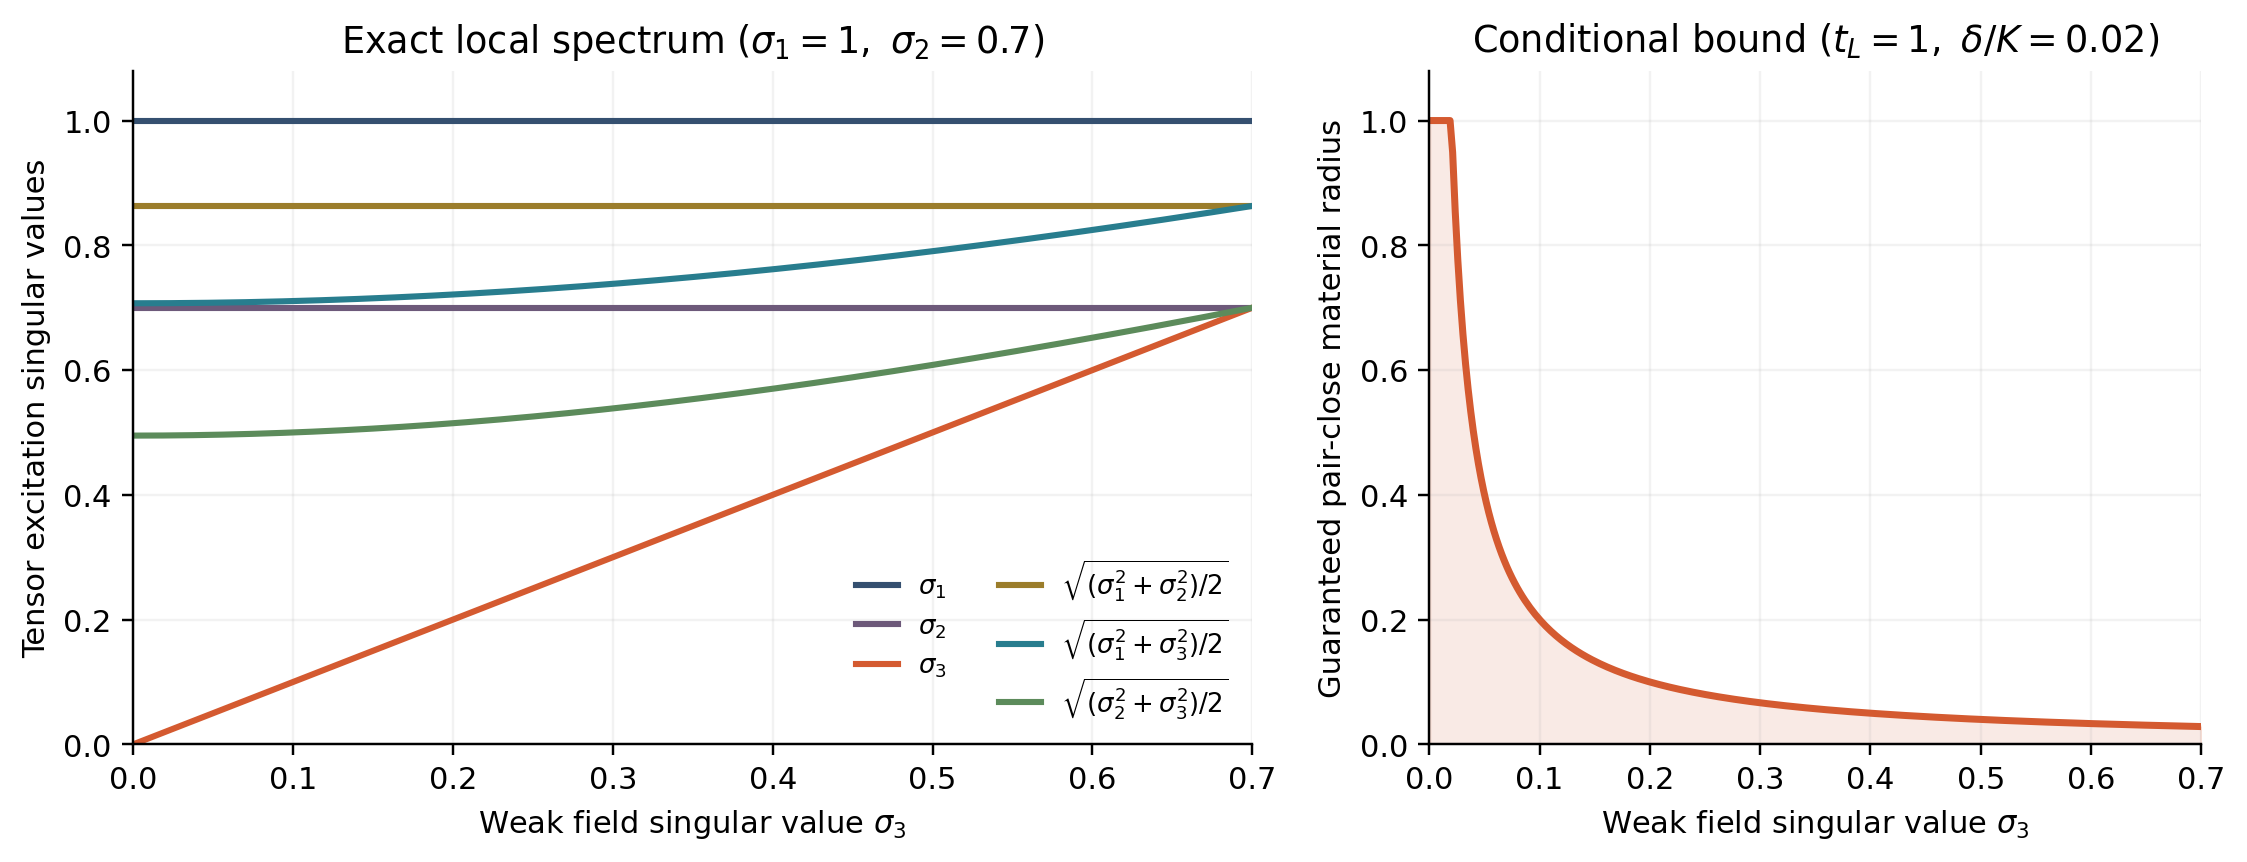
\includegraphics[width=0.98\textwidth,height=\textheight]{figures/tensor_excitation_spectrum.png}
\caption{局部张量激发谱与条件噪声歧义半径。左图严格来自命题
M4；右图采用示意参数
\(t_L=1\)、\(\delta/K=0.02\)，仅展示公式的含义，不是成像实验，也没有估计真实
Maxwell 的 K。}
\end{figure}

\hypertarget{ux8fdeux7eed-maxwell-ux6784ux9020ux4e0eux88abux52a8ux6027}{%
\subsection{6.4 连续 Maxwell
构造与被动性}\label{ux8fdeux7eed-maxwell-ux6784ux9020ux4e0eux88abux52a8ux6027}}

对实对称 SPD 材料，一个复总电场可令

\[
n(x)=\operatorname{Re}E(x)\times\operatorname{Im}E(x),
\qquad \Delta\varepsilon(x)=\alpha(x)n(x)n(x)^T.
\]

取有界非负 \(\alpha\)，紧支撑在源和界面之外的光滑区域，便有
\(\Delta\varepsilon E=0\)。原 \(E,H\) 以及 \(D=\varepsilon E\)
全部不变，curl、Gauss 与辐射条件同时保留。材料仍 SPD；只需更新后 forward
唯一。避免归一化 \(n\) 可以绕开秩变化点除零，但族在 \(n=0\) 处也会退化。

最简单的完整连续反例是背景中的平面波

\[
E=(e_x+i e_y)e^{ikz},\qquad
\varepsilon_r(x)=I+a(x)e_ze_z^T,\quad a(x)\ge0
\]

且 \(a\) 紧支撑。因
\(E_z=0\)，任何这样的有限材料分布都不散射这束波；同传播方向的两个横向偏振仍不能看到
\(\varepsilon_{zz}\)。这不是新的隐身装置定理，而是精确暴露激发盲区的基准。

对两个独立复场可用 \(n=E_1\times E_2\) 构造复对称

\[
\Delta\varepsilon=\kappa f\,\frac{nn^T}{n^*n},
\]

在秩恒定局部区域取光滑 bump
\(f\)。若基准严格被动，\(\operatorname{Im}_H\varepsilon_0\succeq\zeta I\)，扰动范数小于
\(\zeta\)
足以保留被动性；正实部及材料盒还要各自保留裕量。无损边界上任意复方向并不一定合法，不能把``复对称''误写成``自动被动''。

这类有限照明构造与完整边界/全部入射的唯一性不冲突，也不是通常同时变换
\(\varepsilon,\mu\) 的 transformation-optics gauge。最近的直接理论背景是
Guo--Bal
的内部磁场张量重建及其激发秩要求；内部数据不等于这里的外部有限测量。{[}R20{]}

\hypertarget{ux6709ux9650ux566aux58f0ux7684ux4e0dux53efux5206ux8fa8ux534aux5f84}{%
\subsection{6.5
有限噪声的不可分辨半径}\label{ux6709ux9650ux566aux58f0ux7684ux4e0dux53efux5206ux8fa8ux534aux5f84}}

令 \(X_t=X_0+tV\)，\(\|V\|_{\rm mat}=1\)。精确有限差分为

\[
F(X_t)-F(X_0)=tS(I-X_tG)^{-1}VU_0.
\]

设固定数据白化算子为 \(\mathcal W\)，沿合法区间 \(0\le t\le t_L\)
已证明相应接收 resolvent 的诱导范数不超过 \(K\)，则

\[
\|\mathcal W\Delta F\|\le tK\|VU_0\|_F,
\]

\[
\boxed{t_{\rm blind}(\delta)
=\min\left\{t_L,\frac{\delta}{K\|VU_0\|_F}\right\}.}
\]

\(VU_0=0\)
时取整个合法区间。此半径构造了一段有限幅度、全阶多次散射下仍接近的材料族。它给\textbf{逆稳定模量的下界或歧义半径}，不是材料误差上界。

逐格取最弱 dyad \(V_i=h_i\overline p_{i,3}p_{i,3}^*\)，则

\[
\|VU_0\|_F^2=\sum_i|h_i|^2\sigma_{i,3}^2.
\]

在对整个合法集合都有效的同一个 \(K\)
下，可得到不可分辨变化集合的构造性椭球。若 \(K\)
只对一条射线成立，结论也只适用于该射线。近共振可能使 \(K\)
很大，弱激发不再保证有限弱响应；不能用当前 Jacobian
范数替代更新端点的界。

白化噪声上界为 \(\epsilon\) 时，两个预测相距不超过
\(2\epsilon\)，其噪声球可以相交，存在一个观测让二者都合格；任何单点估计至少在其中一个真材料下有不小于材料距离一半的误差。针对已经给定的观测，若
anchor 残差为 \(r_0\)，三角不等式的充分相容条件应为
\(tK\|VU_0\|\le\epsilon-r_0\)。不能把所有 pair-close
材料自动当作当前观测的解；一个不合格 anchor 的同场族仍全部不合格。

\hypertarget{ux4e3aux4ec0ux4e48ux6fc0ux53d1ux6ee1ux79e9ux4ecdux4e0dux80fdux4fddux8bc1ux6750ux6599ux552fux4e00}{%
\subsection{6.6
为什么激发满秩仍不能保证材料唯一}\label{ux4e3aux4ec0ux4e48ux6fc0ux53d1ux6ee1ux79e9ux4ecdux4e0dux80fdux4fddux8bc1ux6750ux6599ux552fux4e00}}

两个向量单元的逻辑反例为

\[
G=0,\quad U_1=U_2=I_3,\quad S=[I_3\ I_3].
\]

材料分别改变 \(+V,-V\)，每个局部激发都满秩，forward
完全稳定，数据却不变。它是有限代数反例，不是具体电磁网格实验。非零耦合下，满足源与接收对称性的空间交换也可给分离材料根；Z-ALG
已有同型历史结构。

因此必须区分：局部激发谱；接收端对可实现注入的下增益；不同有限端点之间的统一可观测性。只有后两者也有严格正下界，才能由局部满秩推出有限材料下稳定界。这与
Atlas 的双端点可观测性同型，不能省略。

\hypertarget{ux65b0ux7167ux660eux4e0eux7b97ux6cd5ux4fddux7559ux89e3ux65cfux5bfbux627eux53efux5206ux7684ux7269ux7406ux95eeux9898}{%
\subsection{6.7
新照明与算法：保留解族，寻找可分的物理问题}\label{ux65b0ux7167ux660eux4e0eux7b97ux6cd5ux4fddux7559ux89e3ux65cfux5bfbux627eux53efux5206ux7684ux7269ux7406ux95eeux9898}}

对已经通过原观测检验的候选 \(X^{(a)}\)，令 \(B\)
是真实可实施的外部发射在成像域产生的入射场矩阵，计算完整传递

\[
\mathcal H_a=S(I-X^{(a)}G)^{-1}X^{(a)}B.
\]

两候选的白化传递差为
\(A_{ab}=W_r(\mathcal H_a-\mathcal H_b)\)。源功率矩阵满足
\(R\succ0\)；冗余源库应先限制到有效发射子空间。在约束 \(c^*Rc\le P_0\)
下，最佳二元辨别由小系统给出：

\[
\max_{c^*Rc\le P_0}\|A_{ab}c\|^2
=P_0\lambda_{\max}(R^{-1/2}A_{ab}^*A_{ab}R^{-1/2}).
\]

这是标准实验设计的应用，不是新的 Rayleigh
商。多候选先用小型物理源库最大化未解决 pair
的最小预测分离即可。若距离超过计入模型误差后的
\(2\epsilon\)，这两个候选不可能同时解释同一个噪声球。局部 rank
增加只破坏同场机制，不保证实际接收区分。

新增源若仅是旧源线性组合，同场族仍不变；物理重测可改善噪声，但应计采集成本。新增频率若共享同一无色散材料，要堆叠所有频率场；未知电导率与介电常数时应共同处理
\((\Delta\varepsilon+i\Delta\sigma/\omega_\ell)U_\ell=0\)，不能逐频随意生成不满足因果色散的张量。

最简单的算法是每格小 SVD、生成合法同场或近同场
dyad、原物理验证、保留材料集合并建议真正能分开的源。无需 NN，也不需要
A17。它改变的是\textbf{如何诚实表示有限照明的信息与不确定性}，不是声称在不可辨识数据上恢复唯一
GT。

与 Z-ALG 的区别必须保留：这里是保持内部状态的显式仿射族；Z-ALG
的孤立根、局部 IFT 图册或分离分支通常有不同内部场。尤其 Z-ALG-E1
已有非置换的连续局部材料图册，本轮不能把``存在连续多解''本身当作项目首次发现。二者可以共同管理候选，却不能被叫作同一个分支生成机制。{[}R36{]}

\hypertarget{ux52a8ux529bux7cfbux7edfux4e13ux9879ux5148ux786eux5b9aux5931ux8d25ux7684ux5bf9ux8c61ux518dux7814ux7a76ux9003ux9038}{%
\section{7.
动力系统专项：先确定失败的对象，再研究逃逸}\label{ux52a8ux529bux7cfbux7edfux4e13ux9879ux5148ux786eux5b9aux5931ux8d25ux7684ux5bf9ux8c61ux518dux7814ux7a76ux9003ux9038}}

\hypertarget{ux4e09ux79cdux7b97ux5b50ux4e0dux80fdux6df7ux4e3aux4e00ux8c08}{%
\subsection{7.1
三种算子不能混为一谈}\label{ux4e09ux79cdux7b97ux5b50ux4e0dux80fdux6df7ux4e3aux4e00ux8c08}}

物理 resolvent \((I-XG)^{-1}\) 描述波的多次散射；\(DF(X)\)
描述材料到数据的一阶敏感性；\(D\mathcal T(z)\)
描述实际算法的一步动态。三者可相关，却不存在``高对比度使 resolvent
大，所以优化必然混沌''的推论。

实际状态应包含材料、电流系数、逐源 PR 梯度与方向、动量、当前
\(\beta\)、活动约束、Fourier
mask、阶段和停止/线搜索状态。参数随迭代变时，使用非自治映射
\(\mathcal T_k\)，或把确定的阶段规则加入扩展状态。只画
\(m_{k+1}=\mathcal T(m_k)\) 可能遗漏决定后续轨迹的历史变量。

仓库证据首先指向预算截断、错误下降几何、活动面和可实现性问题。R3-E
的高成功率轨迹仍大量截断；R4
的更低残差候选可同时具有更差材料。它们都没有给出周期或混沌的证据。{[}R3--R6{]}

\hypertarget{ux4ec0ux4e48ux65f6ux5019ux53efux4ee5ux6392ux9664ux5468ux671fux548c-recurrent-chaos}{%
\subsection{7.2 什么时候可以排除周期和 recurrent
chaos}\label{ux4ec0ux4e48ux65f6ux5019ux53efux4ee5ux6392ux9664ux5468ux671fux548c-recurrent-chaos}}

\textbf{命题 D1（标准 Lyapunov 后果）。} 设 \(K\)
为紧的正向不变集合，\(\mathcal T:K\to K\) 连续，\(V\)
连续，并对所有非固定点满足

\[
V(\mathcal Tz)<V(z).
\]

则每条轨迹的
\(\omega\)-极限集只包含固定点；不存在非平凡有限周期，也不存在由非固定
recurrent 点构成的混沌吸引集合。

\textbf{证明。} \(V(z_k)\) 单调且有下界，故收敛。若聚点 \(z_*\)
不是固定点，连续性给其邻域中一个严格正的单步下降量。轨迹无限次进入该邻域会与
\(V(z_k)\) 收敛矛盾。证毕。

它不保证只收敛到一个点，也不保证那个点是真材料。一个不稳定固定点可有正的线性指数；短时放大也可很强，但这些都不能被叫作一个持续混沌吸引子。

固定单 \(\beta\)、固定 current 空间与权重、每个 block
真正降低同一辅助目标时，CIE 可满足这类 Lyapunov
结构。严格性、连续性、紧性仍须核对。GN
的接受步若对固定原目标严格下降，同样不能具有非平凡的接受状态周期。信赖域内部
trial point 的往返不等于接受轨迹周期。

双
\(\beta\)、阶段改变、动态正则、逐源历史、活动面切换、非精确更新可能破坏共同下降条件；这只是让周期成为数学上可能，并不是观察到它。带过大固定步长的投影梯度甚至能产生边界二周期，但这个普通优化反例不是成熟
CIE 的物理证据。

\hypertarget{ux4e00ux4e2aux5bf9ux53cc-beta-ux89e3ux91caux6709ux7ea6ux675fux529bux7684ux5c40ux90e8ux547dux9898}{%
\subsection{\texorpdfstring{7.3 一个对双 \(\beta\)
解释有约束力的局部命题}{7.3 一个对双 \textbackslash beta 解释有约束力的局部命题}}\label{ux4e00ux4e2aux5bf9ux53cc-beta-ux89e3ux91caux6709ux7ea6ux675fux529bux7684ux5c40ux90e8ux547dux9898}}

在一个可被固定 current
子空间精确表示的无噪物理解附近，先取实标量共享材料、材料盒内点、无正则、每格总场非零。实化
constitutive defect 的微分为

\[
\delta e=B\,\delta a-C\,\delta m,\qquad C^TC=D_q\succ0.
\]

\(C\) 每格对应全部源的真实总场。两块共用的固定正源归一化权重预先吸入
\(B,C\)；\(W_\beta\) 仅表示逐格 CIE
权重，对同一格的各源相同，因而存在对角 \(\Delta_\beta\) 使

\[
W_\beta C=C\Delta_\beta.
\]

材料 readout 在根处的一阶导数为

\[
K_\beta=(C^TW_\beta^2C)^{-1}C^TW_\beta^2B
=D_q^{-1}C^TB.
\]

\textbf{\(\beta_{\rm material}\) 在这个一阶导数中抵消。}
权重本身依赖材料时，根处残差为零使相应导数项消失；离根不成立。

令 current block 使用权重 \(W_j\)，数据微分为 \(A\)，定义

\[
H_{aa}=A^TA+B^TW_j^2B\succ0,\quad
H_{am}=-B^TW_j^2C,\quad H_{mm}=C^TW_j^2C.
\]

\textbf{命题 D2（本轮局部动力学推论）。} 精确 current minimization
后接精确材料 readout，其材料一轮映射的线性化为

\[
M=H_{mm}^{-1}H_{am}^TH_{aa}^{-1}H_{am},
\qquad 0\le\lambda(M)\le1.
\]

\textbf{证明。} 它相似于
\(H_{mm}^{-1/2}H_{am}^TH_{aa}^{-1}H_{am}H_{mm}^{-1/2}\succeq0\)。联合最小二乘
Hessian 为半正定，其 Schur 补给该矩阵不超过
\(I\)。在正定可辨识横向上可严格小于 1。证毕。

因此改变 \(\beta_m\) 不能在这些条件下通过根附近的一阶谱引起 \(-1\) flip
或复共轭单位圆穿越；自然 \(H_{mm}\) 度量下也不存在一步扩张。\(\beta_j\)
可以改变 current block 和收敛速率。实际双 \(\beta\)
的优势应从离物理流形的有限步、截断、正则、活动面或非精确历史中寻找。

这不是全局 CIE 定理。噪声非零残差、未表示的真实
current、节点、材料边界、张量
readout、两块不一致或破坏上述交换结构的权重，以及历史都可能破坏条件。各源数值不同但两块共用的固定正权重，本身不会破坏抵消。Atlas/R3-E
已有 CIE--CSI 缺陷差与 0/2/4 阶结论；本命题是它们与 block
动力学的后果，不能把已有缺陷公式再次列为原创。{[}R4{]}

\hypertarget{ux672cux8f6eux552fux4e00ux5b9eux9645ux8fd0ux884cux7684ux5faeux578bux9a8cux8bc1}{%
\subsection{7.4
本轮唯一实际运行的微型验证}\label{ux672cux8f6eux552fux4e00ux5b9eux9645ux8fd0ux884cux7684ux5faeux578bux9a8cux8bc1}}

提供的 \texttt{dynamics\_toy.py}
使用四材料、三源、三接收的随机复对称代数 VIE，未把其 Green 系数冒充真实
Hankel 网格。保持 \(\beta_j\) 固定，取
\(\beta_m=0.2,1,4\)，根处有限差分导数均匹配上述同一 \(M\)，误差约
\(2.5\times10^{-10}\)。自然度量下四个特征值约为

\[
0.088705,\quad0.137506,\quad0.236844,\quad0.786335.
\]

离根不同 \(\beta_m\) 的 sweep 差表现为 \(O(t^2)\)。脚本和 JSON
原输出随复现包提供。这个检查只排查局部推导的实现错误，不是 full-wave
成像、CIE 性能或原创性证据。

\hypertarget{ux975eux6b63ux89c4ux77acux6001ux5e94ux600eux6837ux6d4b}{%
\subsection{7.5
非正规瞬态应怎样测}\label{ux975eux6b63ux89c4ux77acux6001ux5e94ux600eux6837ux6d4b}}

一个简单矩阵

\[
A=\begin{pmatrix}r&L\\0&r\end{pmatrix},\qquad0<r<1,
\]

有 \(A^k\) 的非对角项
\(kLr^{k-1}\)。所以特征值位于单位圆内仍可出现大有限时放大。这是经典非正规理论，不是
Maxwell 独有的新现象。{[}R25{]}

真实非自治算法应观察

\[
g_{k,h}=\|D\mathcal T_{k+h-1}\cdots D\mathcal T_k\|,
\]

而非逐步特征值。可用少量固定探针、JVP 或小维压缩估计，不必每次形成稠密全
Jacobian。要明确测量的坐标与 metric：命题 D2 说明某些根处 Euclidean
放大只是度量失配；离根、历史和空间切换才可能出现不同机制。

周期证据至少需要完整状态的多次回返、\(p\)
步映射缺陷、多个连续周期及精度/步长复核。持续正 Lyapunov
指数应在固定算法、固定随机序列、充分去掉瞬态之后测量。残差非单调、有限时正指数或
wall 截断末尾振荡都不够。离散周期不能直接称为连续时间极限环。

\hypertarget{ux6e90ux57faux7b49ux53d8ux6027ux540cux4fe1ux606fux7684ux5fc5ux8981ux7a7aux5b9eux9a8c}{%
\subsection{7.6
源基等变性：同信息的必要空实验}\label{ux6e90ux57faux7b49ux53d8ux6027ux540cux4fe1ux606fux7684ux5fc5ux8981ux7a7aux5b9eux9a8c}}

当源共享接收几何时，完整酉变换 \(U_s\in\mathbb C^{p\times p}\) 给

\[
E^{\rm inc}\mapsto E^{\rm inc}U_s,\quad
Y\mapsto YU_s,\quad J\mapsto JU_s,
\]

并严格保留 Frobenius 原物理损失。一般源协方差或权重 \(\Omega\) 应运输为
\(\Omega'=U_s^*\Omega U_s\)。重新逐列归一化通常改变目标，而非只换坐标。

即使同一二次目标，逐源步长也可不等变。例如 Hessian
\(\operatorname{diag}(1,4)\)、两源初始梯度为 \(I\)：逐源精确线搜索产生
\(-\operatorname{diag}(1,1/4)\)；Hadamard 混合后再运输回来得到
\(-0.4I\)，两步相差的 Frobenius 范数约 0.618466。充分解完唯一 current
quadratic
后才恢复正确等变性；有限步交替可能改变后续材料轨迹，但尚无新成像实证。

必须分三臂：原生逐源归一化与 PR；运输完整源 metric 但仍逐源 PR；运输
metric 并采用等变的 global/block update。非对角 \(\Omega'\)
会耦合源，不能继续沿用独立逐源目标而声称完全相同。优化器历史应正确旋转，或所有臂按同一规则重置。

\textbf{查新决定：不把 source remix 主张为新方法。} RMIMO-CSI 和 virtual
experiments 已有直接电磁先例；后者已用数据线性组合来设计 contrast-source
性质。{[}R23--R24{]} 随机压缩到较少 RHS 的 simultaneous-source
方法又是另一类既有机制，它改变单次目标的噪声/cross-talk，不能与保留全部列的酉空实验混用。

\hypertarget{ux662fux5426ux5b58ux5728ux5ec9ux4ef7ux7684ux9519ux8bef-basin-ux4fe1ux53f7}{%
\subsection{7.7 是否存在廉价的错误 basin
信号}\label{ux662fux5426ux5b58ux5728ux5ec9ux4ef7ux7684ux9519ux8bef-basin-ux4fe1ux53f7}}

没有一个仅靠相同数据和相同先验、普遍知道``哪一个合法解才是生成
GT''的判据；命题 M3 已给严格反例。可以检测的对象更窄：

\begin{longtable}[]{@{}
  >{\raggedright\arraybackslash}p{(\columnwidth - 4\tabcolsep) * \real{0.3333}}
  >{\raggedright\arraybackslash}p{(\columnwidth - 4\tabcolsep) * \real{0.3333}}
  >{\raggedright\arraybackslash}p{(\columnwidth - 4\tabcolsep) * \real{0.3333}}@{}}
\toprule\noalign{}
\begin{minipage}[b]{\linewidth}\raggedright
可记录量
\end{minipage} & \begin{minipage}[b]{\linewidth}\raggedright
能支持的解释
\end{minipage} & \begin{minipage}[b]{\linewidth}\raggedright
不能推出
\end{minipage} \\
\midrule\noalign{}
\endhead
\bottomrule\noalign{}
\endlastfoot
原物理 discrepancy、constitutive defect & 是否具备数据/物理资格 &
已达到真实材料 \\
projected gradient、KKT 缺陷 & 约束一阶停滞 & 全局最优 \\
活动面及 free Hessian & 面内曲率与边界锁定 & 全临界锥严格局部最优 \\
current 表示误差及空间扩张收益 & 是否可能有容量瓶颈 &
必然是唯一失败原因 \\
实际/预测下降比 & 局部模型是否可信 & 可信下降方向接近 GT \\
完整状态有限时放大 & 算法局部敏感与瞬态 & 混沌或错误性 \\
合法候选的新照明预测差 & 候选之间可能被何种数据区分 & 已经获得新信息 \\
\end{longtable}

最简单规则是：在预先声明的物理不合格与停滞条件共同满足时，触发一个来自独立结构的有限候选；同时给成熟
CIE
续跑、空间扩张与同费用普通扰动机会。此触发只称``停滞事件''，不称自动识别错误
basin。若实测多数失败是稳定固定点，就终止混沌路线，转向支撑信息、状态容量或新增照明。

\hypertarget{ux5176ux4ed6ux7ed3ux6784ux54eaux4e9bux503cux5f97ux4fddux7559ux54eaux4e9bux5e94ux964dux7ea7}{%
\section{8.
其他结构：哪些值得保留，哪些应降级}\label{ux5176ux4ed6ux7ed3ux6784ux54eaux4e9bux503cux5f97ux4fddux7559ux54eaux4e9bux5e94ux964dux7ea7}}

\hypertarget{ux56e0ux679cux6570ux636eux7684ux5185ux90e8-gramux591aux6b21ux6563ux5c04ux4e0dux53eaux662fux9ebbux70e6}{%
\subsection{8.1 因果数据的内部
Gram：多次散射不只是麻烦}\label{ux56e0ux679cux6570ux636eux7684ux5185ux90e8-gramux591aux6b21ux6563ux5c04ux4e0dux53eaux662fux9ebbux70e6}}

在无损、自伴、同置收发的适当能量变量下，设波算子 \(A\succeq0\)，源注入
\(B\)，时间快照 \(U_j=\cos(j\tau\sqrt A)B\)，数据为

\[
D_j=B^*\cos(j\tau\sqrt A)B.
\]

余弦乘积直接给

\[
M_{ij}=U_i^*U_j
=\tfrac12(D_{i+j}+D_{|i-j|}).
\]

相邻传播的 Gram 也由四个相邻数据时刻的组合得到。快照独立、\(M\succ0\)
时，令 \(M=R^*R\)，投影传播矩阵可由相应 Gram \(K\) 构成
\(R^{-*}KR^{-1}\)。秩亏时必须明示截断，并仅在保留空间取逆。这类数据 ROM
利用了所有已到达的多次散射，而不需要先知道材料再计算其 Jacobian。

这是已建立的路线。Borcea--Liu--Zimmerling 的 2024
电磁论文已有各向异性、二维矢量、沿一方向不变的模型；不能描述成已经完成任意三维张量
Maxwell。{[}R14{]} 数据 Gram 的恒等式与把 ROM 基 lift 到物理空间的参考
kinematics 近似，也必须分开。

本项目更有价值的开放点是非同置矩形数据、有限孔径和损耗下哪些交叉 Gram
可稳定恢复。损耗层状 ROM
已有先例，不能泛称``加入损耗''就是创新。{[}R15{]} \(m\) 端口、\(n\)
时间块的全 Gram 若做稠密 Cholesky，费用约
\(O((mn)^3)\)；三维大量端口必须先解决局部/分块压缩。

它可以产生与当前错误材料形状无关的内部状态约束，因而有机会改变
basin；但同数据的成熟 multi-frequency CIE
必须拿到同样的宽带信息。更多频率本身的收益不得归入 ROM 算法。

\hypertarget{ux6750ux6599ux4ee3ux6570ux5171ux540cux95edux5305ux56faux5b9aux7a7aux95f4ux6210ux7acbux7684ux6b63ux786eux6761ux4ef6}{%
\subsection{8.2
材料代数共同闭包：固定空间成立的正确条件}\label{ux6750ux6599ux4ee3ux6570ux5171ux540cux95edux5305ux56faux5b9aux7a7aux95f4ux6210ux7acbux7684ux6b63ux786eux6761ux4ef6}}

设合法材料只有 \(k\) 个已知分区参数，\(X(d)=\sum_{a=1}^kd_aP_a\)。令
\(A_a=P_aG\)、\(B_a=P_aE^{\rm inc}\)，构造

\[
\mathcal U_0=\operatorname{span}\{B_a\},\qquad
\mathcal U_{j+1}=\mathcal U_j+\sum_aA_a\mathcal U_j.
\]

在有限空间停止后，\(\mathcal U\) 同时包含注入且对全部 \(A_a\) 不变。若
\(V\) 是其正交基，原 forward 可逆，则电流严格位于 \(\mathcal U\)，满足

\[
\left(I-\sum_ad_aV^*A_aV\right)\widehat J
=\sum_ad_aV^*B_a,\qquad J=V\widehat J.
\]

证明只需限制到不变子空间，完全不要求目标材料处 Neumann
级数收敛。它体现的是\textbf{材料乘法与传播交错生成的代数}，而非单个
\(G\) 的谱。该思想属于 bilinear/parametric realization 的应用。{[}R21{]}

静态参数彼此交换，数据 Taylor 系数只决定 word
的对称和；不能把上述足够闭包误称静态多参数响应的最小 McMillan
实现。标量自由像素且每行受激时，初始闭包已满张成；向量情形还取决于各格激发秩及后续传播闭包。单幅度回到
Atlas
已有结果。合适探索对象是分层、镜面对称团簇和周期超胞；轻微非对称、新极化和近共振是必要反例。

\hypertarget{ux5b8cux6574ux6563ux5c04ux77e9ux9635ux7684ux6f0fux6d4bux80fdux91cf-gram}{%
\subsection{8.3 完整散射矩阵的漏测能量
Gram}\label{ux5b8cux6574ux6563ux5c04ux77e9ux9635ux7684ux6f0fux6d4bux80fdux91cf-gram}}

对正确功率归一化的无损完整散射矩阵
\(\mathscr S\)，\(\mathscr S^*\mathscr S=I\)。将输入输出分成已测 \(P\)
和遗漏 \(Q\)，令 \(A=\mathscr S_{PP}\)，则

\[
\mathscr S_{QP}^*\mathscr S_{QP}=I-A^*A.
\]

所以共置已测子块决定漏测输出的输入空间
Gram、非零奇异值及组合入射的漏出功率，但不决定输出相位和左奇异向量。有损被动情况变成

\[
I-A^*A=\mathscr S_{QP}^*\mathscr S_{QP}+\mathcal A_P,
\qquad\mathcal A_P\succeq0,
\]

漏测与吸收无法仅由 \(A\) 分开。误差 \(\|\widetilde A-A\|\le\nu\) 给 Gram
误差至多 \(2\nu+\nu^2\)，可据此给稳健的隐藏通道秩下界。

这些是标准 block-unitary 与扰动后果。它们有助于 lifted response、NN
completion 和 ROM 最低阶数诊断；对已经满足完整无损 Maxwell 且拟合 \(A\)
的材料，约束自动成立，不能再次用于选出 GT。普通矩形 point-receiver
的散射场矩阵也不自动等于这个功率散射子块。

\hypertarget{ux975eux5c40ux90e8ux8054ux5408ux53d8ux5316ux54eaux4e9bux4e00ux9636ux76f2ux533aux6709ux9ad8ux9636ux4fe1ux53f7}{%
\subsection{8.4
非局部联合变化：哪些一阶盲区有高阶信号}\label{ux975eux5c40ux90e8ux8054ux5408ux53d8ux5316ux54eaux4e9bux4e00ux9636ux76f2ux533aux6709ux9ad8ux9636ux4fe1ux53f7}}

一个精确两单元模型，\(G_{12}=G_{21}=g\)、\(G_{11}=G_{22}=0\)，入射
\((1,0)^T\)、接收行 \((0,1)\)，给

\[
F(d_1,d_2)=\frac{g d_1d_2}{1-g^2d_1d_2}.
\]

从零材料出发单独增加任一区域都没有响应，联合变化才显现。这是标准多次散射路径，不是新恒等式，也不能把抽象端口系数当真实布置。它能作为决定性机制设计：利用物理端口组合形成近似隔离激发/接收，然后加入完整原通道检查该合作信号仍有价值。

与同场族的区别是：这里只有初始一阶材料数据导数为零，联合方向的
\(\Delta XU\)
并不持续为零。若要据此生成候选，必须有独立物理理由选择两个区域，而不只是再作指数级块搜索。精确有限响应和小支持
Woodbury 已由 Atlas
覆盖；目前没有证据表明给它们换成``散射闭环''的名称就能超越成熟 CIE。

\hypertarget{ux4e24ux6761ux771fux6b63ux4e0dux540cux4f46ux4e0dux80fdux5938ux5927ux7684ux8c31ux8defux7ebf}{%
\subsection{8.5
两条真正不同、但不能夸大的谱路线}\label{ux4e24ux6761ux771fux6b63ux4e0dux540cux4f46ux4e0dux80fdux5938ux5927ux7684ux8c31ux8defux7ebf}}

Griesmaier--Hanke 2025 已给基于低阶远场 Fourier
系数、虚拟原点和有理逼近的 one-shot 定位方法，原理论针对二维标量
Helmholtz 中特定分离源/散射体的位置。{[}R22{]}
它为与当前错误材料无关的粗支撑 proposal
提供候选工具，不能直接恢复一般高对比度材料、内部空腔或密集耦合的任意形状，也不能未经推导推广成三维矢量定理。研究价值在其适用边界与后续全波
corrector 的同成本表现，不能称``首次用 Fourier 找全局 basin''。

CGO、D-bar
与非线性散射变换也表明，某些逆问题可以把非线性转移到一个特殊数据变换再作空间恢复。{[}R31{]}
但在有限孔径、有限频率、矢量 Maxwell
中，构造该变换可能需要不稳定延拓或高成本的辅助问题。其理论价值很高，当前实用优先级低；不能把标量二维或完整边界定理直接搬成强散射一次
IFFT。

\hypertarget{nn-ux7684ux4f4dux7f6eux4e0eux5fc5ux8981ux7684ux5426ux8bc1ux5b9eux9a8c}{%
\subsection{8.6 NN
的位置与必要的否证实验}\label{nn-ux7684ux4f4dux7f6eux4e0eux5fc5ux8981ux7684ux5426ux8bc1ux5b9eux9a8c}}

前三条主线的首个决定性实验均不需要
NN。只有明确的解析变量已通过机制门槛后，才考虑小网络预测：磁场的少量状态系数；数据
ROM
的局部补全；有限个支撑拓扑；可实现的张量自由参数。输出必须经合法材料检查和完整
Maxwell 验证。

如果网络沿严格同场方向选择材料，它使用的是训练先验，不能说观测识别了这些分量。若用训练分布学习形状，则应把相同先验用于成熟
CIE 的初始化/正则对照，并把离线 forward、训练样本和训练费用单列。

至少设四个相同候选数/校正成本的 proposal
对照：解析结构；随机但同合法域；一般小网络；结构条件小网络。测试按几何族、对比度、源/极化和材料类别划分，而非只换九数字像素。在线不读取测试
GT；不能用 best@K 的 GT oracle 代替最终 top-1
选择。若结构网络只在固定训练形状有利、与一般网络无差异，应归因为先验学习，而非新
Maxwell 机制。

\hypertarget{ux65b0ux7406ux8bbaux4e0eux7b97ux6cd5ux5019ux9009ux5b8cux6574ux6bd4ux8f83ux5361}{%
\section{9.
新理论与算法候选完整比较卡}\label{ux65b0ux7406ux8bbaux4e0eux7b97ux6cd5ux5019ux9009ux5b8cux6574ux6bd4ux8f83ux5361}}

每张卡覆盖变量、非线性、子空间、非局部搜索、NN、CIE
区别、数学目标、费用、病态与否证。各候选不是同一方法的参数变体。

\Needspace{18\baselineskip}

\hypertarget{m1ux56faux5b9aux78c1ux573aux5408ux6cd5ux7a7aux95f4ux4e0eux6750ux6599-hodge-ux573aux65cf}{%
\subsection{M1：固定磁场合法空间与材料 Hodge
场族}\label{m1ux56faux5b9aux78c1ux573aux5408ux6cd5ux7a7aux95f4ux4e0eux6750ux6599-hodge-ux573aux65cf}}

\begin{longtable}[]{@{}
  >{\raggedright\arraybackslash}p{(\columnwidth - 2\tabcolsep) * \real{0.2450}}
  >{\raggedright\arraybackslash}p{(\columnwidth - 2\tabcolsep) * \real{0.7550}}@{}}
\toprule\noalign{}
\begin{minipage}[b]{\linewidth}\raggedright
维度
\end{minipage} & \begin{minipage}[b]{\linewidth}\raggedright
判断
\end{minipage} \\
\midrule\noalign{}
\endhead
\bottomrule\noalign{}
\endlastfoot
核心结构 / 新变量 & 已知 \(\mu\) 下固定无散
\(H\)；\(\eta=\varepsilon^{-1}\)；电场以材料 lift 恢复 \\
非线性 / 子空间 & 保留材料与场耦合；固定横向基或随材料合法 lift，绝非全
resolvent 共同谱 \\
非局部 / NN & 小维场释放可提议材料；NN 暂不需要 \\
与 CIE / 前人 & 比较物理状态表示，不是新交替最小化；CSI/WRI、PVIE、Hodge
均为先例 \\
数学可能性 & 能量宽度、界面正则、lift 变化界、端口/弱残差控制 \\
成本 / 病态 & curl 局部应用；Hodge
需变系数椭圆解；边界消元和共振不可省略 \\
决定实验 / 优先级 & 3D gap/薄壳，等模式与等总成本对四表示；主线，若普通
H 已够则删复杂 lift \\
\end{longtable}

\Needspace{18\baselineskip}

\hypertarget{m2ux6709ux9650ux901aux9053ux5168ux6ce2ux5355ux8c03ux6027ux6392ux9664}{%
\subsection{M2：有限通道全波单调性排除}\label{m2ux6709ux9650ux901aux9053ux5168ux6ce2ux5355ux8c03ux6027ux6392ux9664}}

\begin{longtable}[]{@{}
  >{\raggedright\arraybackslash}p{(\columnwidth - 2\tabcolsep) * \real{0.2450}}
  >{\raggedright\arraybackslash}p{(\columnwidth - 2\tabcolsep) * \real{0.7550}}@{}}
\toprule\noalign{}
\begin{minipage}[b]{\linewidth}\raggedright
维度
\end{minipage} & \begin{minipage}[b]{\linewidth}\raggedright
判断
\end{minipage} \\
\midrule\noalign{}
\endhead
\bottomrule\noalign{}
\endlastfoot
核心结构 / 新变量 & 远场谱序和探测块；先处理支撑假说 \\
非线性 / 子空间 & 完整全波响应；通道压缩而非当前材料切空间 \\
非局部 / NN & 排除部分支撑假说后生成拓扑候选；NN 不需要 \\
与 CIE / 前人 & 全局序约束不同于局部数据下降；2023 Maxwell、2026
Helmholtz 已有基础 \\
数学可能性 & 可用的统一例外数、噪声界、有限孔径证书或不可能性区域 \\
成本 / 病态 & 预计算探测
Gram，小矩阵谱；\(k\ge p\)、校准、失配、弱特征值可使无效 \\
决定实验 / 优先级 & 已知零背景、连通补集、固定测量；未知 \(k\)
立即降级；理论主线 \\
\end{longtable}

\Needspace{18\baselineskip}

\hypertarget{m3ux6709ux9650ux7167ux660eux7684ux5f20ux91cfux53efux89c2ux6d4bux5546}{%
\subsection{M3：有限照明的张量可观测商}\label{m3ux6709ux9650ux7167ux660eux7684ux5f20ux91cfux53efux89c2ux6d4bux5546}}

\begin{longtable}[]{@{}
  >{\raggedright\arraybackslash}p{(\columnwidth - 2\tabcolsep) * \real{0.2450}}
  >{\raggedright\arraybackslash}p{(\columnwidth - 2\tabcolsep) * \real{0.7550}}@{}}
\toprule\noalign{}
\begin{minipage}[b]{\linewidth}\raggedright
维度
\end{minipage} & \begin{minipage}[b]{\linewidth}\raggedright
判断
\end{minipage} \\
\midrule\noalign{}
\endhead
\bottomrule\noalign{}
\endlastfoot
核心结构 / 新变量 & \(\Delta\chi_iU_i=0\) 的同场族与六项激发谱 \\
非线性 / 子空间 & 该族保留全部多次散射且无需线性化；每格激发核随 anchor
场变化 \\
非局部 / NN & 有限合法张量族、主动新源；NN 只能提供先验选择 \\
与 CIE / 前人 &
描述信息缺失，不是更强局部求解；内部张量重建与各向异性唯一性为邻近理论 \\
数学可能性 & 连续族正则性、噪声歧义半径、共享色散与最少照明条件 \\
成本 / 病态 & 每格 \(3\times s\) 小 SVD；秩变化、passivity 边界、弱场与
receiver cancellation \\
决定实验 / 优先级 & 独立网格同场确认、加接收无效、新源全波分离；理论与
benchmark 高优先 \\
\end{longtable}

\Needspace{18\baselineskip}

\hypertarget{m4ux6709ux9650ux5b54ux5f84ux4e0eux635fux8017ux4e0bux7684ux56e0ux679cux6570ux636e-rom}{%
\subsection{M4：有限孔径与损耗下的因果数据
ROM}\label{m4ux6709ux9650ux5b54ux5f84ux4e0eux635fux8017ux4e0bux7684ux56e0ux679cux6570ux636e-rom}}

\begin{longtable}[]{@{}
  >{\raggedright\arraybackslash}p{(\columnwidth - 2\tabcolsep) * \real{0.2450}}
  >{\raggedright\arraybackslash}p{(\columnwidth - 2\tabcolsep) * \real{0.7550}}@{}}
\toprule\noalign{}
\begin{minipage}[b]{\linewidth}\raggedright
维度
\end{minipage} & \begin{minipage}[b]{\linewidth}\raggedright
判断
\end{minipage} \\
\midrule\noalign{}
\endhead
\bottomrule\noalign{}
\endlastfoot
核心结构 / 新变量 & 数据决定内部时间快照 Gram 与投影传播矩阵 \\
非线性 / 子空间 & 将多次散射迁移到数据状态表示；空间基 lift
可能是近似 \\
非局部 / NN & ROM 约束的场/材料候选；小网络仅辅助缺失 Gram，非必要 \\
与 CIE / 前人 & 目标可由数据状态结构组织；已有直接 2024 二维各向异性 EM
ROM \\
数学可能性 & 非同置/有损交叉 Gram 的可辨识性、局部 ROM 一致性与稳定性 \\
成本 / 病态 & 全 Gram 稠密分解可达
\(O((mn)^3)\)；小奇异值噪声放大与相位/时间校准 \\
决定实验 / 优先级 & 一维层状→二维 TE；所有臂同宽带数据；战略备选 \\
\end{longtable}

\Needspace{18\baselineskip}

\hypertarget{m5ux6750ux6599ux4ee3ux6570ux7684ux5171ux540cux4f20ux64adux95edux5305}{%
\subsection{M5：材料代数的共同传播闭包}\label{m5ux6750ux6599ux4ee3ux6570ux7684ux5171ux540cux4f20ux64adux95edux5305}}

\begin{longtable}[]{@{}
  >{\raggedright\arraybackslash}p{(\columnwidth - 2\tabcolsep) * \real{0.2450}}
  >{\raggedright\arraybackslash}p{(\columnwidth - 2\tabcolsep) * \real{0.7550}}@{}}
\toprule\noalign{}
\begin{minipage}[b]{\linewidth}\raggedright
维度
\end{minipage} & \begin{minipage}[b]{\linewidth}\raggedright
判断
\end{minipage} \\
\midrule\noalign{}
\endhead
\bottomrule\noalign{}
\endlastfoot
核心结构 / 新变量 & \(\{P_aG\}\) 与源注入生成的共同不变子空间 \\
非线性 / 子空间 & 在闭包中精确保留参数
resolvent；固定但只对声明材料类有效 \\
非局部 / NN & 小系统查询多分区材料候选；不需要 NN \\
与 CIE / 前人 & 利用具体材料代数而非通用 Fourier；bilinear/parametric
MOR 已有 \\
数学可能性 & 对称/分区的最小足够状态、近可约性与端口误差 \\
成本 / 病态 & 离线闭包可能长到全 \(N\)；近共振使小非对称扰动被放大 \\
决定实验 / 优先级 &
对称双体→轻微破缺→新照明；中优先，不能强制低维材料造收益 \\
\end{longtable}

\Needspace{18\baselineskip}

\hypertarget{m6ux6f0fux6d4bux80fdux91cf-gram-ux4e0eux5c40ux57dfux5b9eux73b0ux6027}{%
\subsection{M6：漏测能量 Gram
与局域实现性}\label{m6ux6f0fux6d4bux80fdux91cf-gram-ux4e0eux5c40ux57dfux5b9eux73b0ux6027}}

\begin{longtable}[]{@{}
  >{\raggedright\arraybackslash}p{(\columnwidth - 2\tabcolsep) * \real{0.2450}}
  >{\raggedright\arraybackslash}p{(\columnwidth - 2\tabcolsep) * \real{0.7550}}@{}}
\toprule\noalign{}
\begin{minipage}[b]{\linewidth}\raggedright
维度
\end{minipage} & \begin{minipage}[b]{\linewidth}\raggedright
判断
\end{minipage} \\
\midrule\noalign{}
\endhead
\bottomrule\noalign{}
\endlastfoot
核心结构 / 新变量 & \(I-A^*A\) 与隐藏通道响应；power-normalized
completion \\
非线性 / 子空间 & 非线性迁移到局域材料实现性；无需材料切空间 \\
非局部 / NN & 可约束 lifted response/NN
补全，不直接区分完整物理同数据材料 \\
与 CIE / 前人 & standard unitary dilation/optical-theorem
结构；不是增加测量信息 \\
数学可能性 & 哪些被动响应补全可由局域 Maxwell 材料实现 \\
成本 / 病态 & 端口小 Gram；漏测与吸收不可分、通道归一化错误 \\
决定实验 / 优先级 & 无损/有损同几何，验证能量诊断及反例；辅助低优先 \\
\end{longtable}

\Needspace{18\baselineskip}

\hypertarget{m7ux865aux62dfux539fux70b9ux4e0eux4f4eux9636-fourier-ux6709ux7406ux5b9aux4f4d}{%
\subsection{M7：虚拟原点与低阶 Fourier
有理定位}\label{m7ux865aux62dfux539fux70b9ux4e0eux4f4eux9636-fourier-ux6709ux7406ux5b9aux4f4d}}

\begin{longtable}[]{@{}
  >{\raggedright\arraybackslash}p{(\columnwidth - 2\tabcolsep) * \real{0.2450}}
  >{\raggedright\arraybackslash}p{(\columnwidth - 2\tabcolsep) * \real{0.7550}}@{}}
\toprule\noalign{}
\begin{minipage}[b]{\linewidth}\raggedright
维度
\end{minipage} & \begin{minipage}[b]{\linewidth}\raggedright
判断
\end{minipage} \\
\midrule\noalign{}
\endhead
\bottomrule\noalign{}
\endlastfoot
核心结构 / 新变量 & 少数分离散射体的空间位置与远场低阶 Fourier 系数 \\
非线性 / 子空间 & 用源等效/渐近结构处理定位，不解决一般完整材料非线性 \\
非局部 / NN & 与当前材料无关的位置 proposal；NN 不需要 \\
与 CIE / 前人 & 2025 one-shot
方法已存在；本项目只能研究强耦合边界与后续校正 \\
数学可能性 & 分离尺度、噪声与强多次散射下的位置稳定性 \\
成本 / 病态 & 少量系数和有理拟合；目标重叠、近零、有限孔径使不稳定 \\
决定实验 / 优先级 & 两体逐渐靠近，普通定位基线与同成本 CIE；有限备选 \\
\end{longtable}

\Needspace{18\baselineskip}

\hypertarget{m8ux975eux7ebfux6027ux6563ux5c04ux53d8ux6362-cgo-d-bar}{%
\subsection{M8：非线性散射变换 / CGO /
D-bar}\label{m8ux975eux7ebfux6027ux6563ux5c04ux53d8ux6362-cgo-d-bar}}

\begin{longtable}[]{@{}
  >{\raggedright\arraybackslash}p{(\columnwidth - 2\tabcolsep) * \real{0.2450}}
  >{\raggedright\arraybackslash}p{(\columnwidth - 2\tabcolsep) * \real{0.7550}}@{}}
\toprule\noalign{}
\begin{minipage}[b]{\linewidth}\raggedright
维度
\end{minipage} & \begin{minipage}[b]{\linewidth}\raggedright
判断
\end{minipage} \\
\midrule\noalign{}
\endhead
\bottomrule\noalign{}
\endlastfoot
核心结构 / 新变量 & 特殊复几何光学解与非线性散射数据 \\
非线性 / 子空间 & 将非线性转移到数据变换；非一般材料低秩投影 \\
非局部 / NN & 可产生直接全局候选；NN 非必需，不能代替稳定性 \\
与 CIE / 前人 & 经典 inverse-scattering 非线性 Fourier
理论，和优化路线不同 \\
数学可能性 & 有限可测通道的稳定截断、被动矢量推广与不可能性 \\
成本 / 病态 & 复杂频率/解析延拓、辅助 PDE、强噪声放大 \\
决定实验 / 优先级 & 先完整数据特殊模型，失败于有限孔径即止；理论储备 \\
\end{longtable}

\Needspace{18\baselineskip}

\hypertarget{m9cie-ux6e90ux57faux7b49ux53d8ux6027ux4e0eux5c40ux90e8ux52a8ux6001ux9650ux5236}{%
\subsection{M9：CIE
源基等变性与局部动态限制}\label{m9cie-ux6e90ux57faux7b49ux53d8ux6027ux4e0eux5c40ux90e8ux52a8ux6001ux9650ux5236}}

\begin{longtable}[]{@{}
  >{\raggedright\arraybackslash}p{(\columnwidth - 2\tabcolsep) * \real{0.2450}}
  >{\raggedright\arraybackslash}p{(\columnwidth - 2\tabcolsep) * \real{0.7550}}@{}}
\toprule\noalign{}
\begin{minipage}[b]{\linewidth}\raggedright
维度
\end{minipage} & \begin{minipage}[b]{\linewidth}\raggedright
判断
\end{minipage} \\
\midrule\noalign{}
\endhead
\bottomrule\noalign{}
\endlastfoot
核心结构 / 新变量 & 完整迭代状态、源 metric 与等变性；根处 \(\beta_m\)
抵消 \\
非线性 / 子空间 & 原物理不变，研究算法坐标/历史；源列空间不变 \\
非局部 / NN & 轨迹扰动只能作 globalization，不增加信息；NN 暂不需要 \\
与 CIE / 前人 & RMIMO-CSI/virtual experiments
已有；新点只能是审计与条件排除 \\
数学可能性 & 非自治有限时界、活动面转换、真实算法的等变条件 \\
成本 / 病态 & 少量重放/JVP；完整 history 与 covariance 易遗漏 \\
决定实验 / 优先级 &
三臂源基空实验及根附近导数；必做低成本诊断，非主成像论文 \\
\end{longtable}

\hypertarget{ux6700ux5c0fux51b3ux5b9aux6027ux5b9eux9a8cux4e0eux65b0ux7684ux7269ux7406-benchmark}{%
\section{10. 最小决定性实验与新的物理
benchmark}\label{ux6700ux5c0fux51b3ux5b9aux6027ux5b9eux9a8cux4e0eux65b0ux7684ux7269ux7406-benchmark}}

\hypertarget{ux5148ux505aux80fdux6539ux53d8ux7814ux7a76ux51b3ux7b56ux7684ux5b9eux9a8c}{%
\subsection{10.1
先做能改变研究决策的实验}\label{ux5148ux505aux80fdux6539ux53d8ux7814ux7a76ux51b3ux7b56ux7684ux5b9eux9a8c}}

本报告不要求每条方向都走完小模型、二维、三维和大量新目标。最小实验的任务是消除一个关键不确定性，而不是积累数量。所有新成像先有机制证据，再冻结选择器与预算合同，最后进行新鲜材料确认。

\begin{longtable}[]{@{}
  >{\raggedright\arraybackslash}p{(\columnwidth - 6\tabcolsep) * \real{0.2500}}
  >{\raggedright\arraybackslash}p{(\columnwidth - 6\tabcolsep) * \real{0.2500}}
  >{\raggedright\arraybackslash}p{(\columnwidth - 6\tabcolsep) * \real{0.2500}}
  >{\raggedright\arraybackslash}p{(\columnwidth - 6\tabcolsep) * \real{0.2500}}@{}}
\toprule\noalign{}
\begin{minipage}[b]{\linewidth}\raggedright
实验
\end{minipage} & \begin{minipage}[b]{\linewidth}\raggedright
最小物理模型与控制量
\end{minipage} & \begin{minipage}[b]{\linewidth}\raggedright
支持机制的结果
\end{minipage} & \begin{minipage}[b]{\linewidth}\raggedright
推翻、降级或停止条件
\end{minipage} \\
\midrule\noalign{}
\endhead
\bottomrule\noalign{}
\endlastfoot
E1 场表示 & 已知 \(\mu\) 的 3D 正介电双体，先仅改变 gap & 同 DOF
与总费用下，磁场或 lift 同时改善 curl、端口和状态缺陷 & 只降低 \(H\) 的
\(L^2\) 误差；优势被普通 CIE 扩模解释 \\
E2 单调性资格 & 规则实心体，已知零背景，配对远场通道 & 有独立
\(k<p\)、有效 \(\delta\)，可稳健拒绝错误包含假设 & \(k\) 未知或
\(k\ge p\)；误差界靠 GT；矩形近场被误用 \\
E3 精确张量族 & 一个公开开发锚点，实对称与严格被动复对称各一例 &
显著材料变化保持旧源全部场；独立网格误差收敛 &
合法性失败或仅粗离散身份成立；不能升级成连续结论 \\
E4 主动区分 & E3 同场族与小型真实源库 &
真实新源的全波预测分离超过噪声；旧源重组仍不可分 & 只增加局部
rank、实际端口差仍小；不得称解决多解 \\
E5 CIE 动态 & 公开根局部检查，再一个成功和一个失败历史例 & \(\beta_m\)
一阶抵消；失败归类到具体阶段/活动面/预算 &
真实条件满足而导数不同；先查推导接线，不继续宣传 \\
E6 源基空实验 & 同一完整 \(E,Y\) 的三个预定酉基 &
三臂区分目标改变与纯历史/坐标效应 & 不运输
covariance；只报早期加速而称新信息 \\
E7 因果 ROM & 一维层状→二维矢量，所有臂同宽带数据 & 可用 Gram 或局部 ROM
在相同数据上改善状态恢复 & 强噪声需不稳定补全；稠密成本吞没收益 \\
E8 共同闭包 & 已知分区、对称双体，逐步破坏对称 &
小闭包与实际端口误差在明确范围稳定 & 自由像素立即全秩；强制减材料 DOF
才得到收益 \\
\end{longtable}

E1 的第一步不需要先重写完整磁场反演器。用可信全矢量 forward 得到
\(E,H,J\)，先比较背景/开发材料构造的固定基与离线 oracle
最佳表示；它能最便宜地否定``磁场更小''假说。只有信号清楚，才实现辅助场
proposal。

E3
也不需要在不可辨识问题上训练网络或反复优化。解析同场构造先回答``数据可不可能区分''，然后才决定该任务应输出一个材料、一个等价类，还是下一次照明建议。

\hypertarget{ux516dux7c7bux503cux5f97ux8fdbux5165ux6210ux50cfux9636ux6bb5ux7684ux573aux666f}{%
\subsection{10.2
六类值得进入成像阶段的场景}\label{ux516dux7c7bux503cux5f97ux8fdbux5165ux6210ux50cfux9636ux6bb5ux7684ux573aux666f}}

\textbf{场景 A：高对比双体与可控窄缝。}
固定体积、形状、材料、频率和源，只改变间距。数学难点是相互耦合、界面电荷及高空间频率
current。先与单体和大间距控制比较；记录 current Fourier
表示误差、\(H(\operatorname{curl})\) 误差与原数据
discrepancy。正例应显示表示改善转化为材料或同精度成本改善，而不是因为增加总模式或
correction 次数。无需 NN。

\textbf{场景 B：三维薄壳、偏心空腔与通孔。}
分别改变壳厚或偏心率，不同时增大电尺寸。它们检验界面场表示与内部电流结构，适合
M1；封闭壳的拓扑可能不满足
M2，必须分别标资格。以同外形实心体、同材料体积的开放结构作控制。除了张量/标量
NRMSE，报告空腔是否由数据区分及重新网格化后的端口预测。

\textbf{场景 C：低损耗内部共振。}
固定几何，少量预定频率或损耗值使其接近/离开内部共振；先由公开 forward
诊断选物理区间，不能看测试反演结果后选最有利频点。记录
resolvent/线性求解难度、原物理导数及算法有限时放大，三者分开。比较所有方法使用同一复材料类别；real-only
CIE 的模型缺失不是算法失败。

\textbf{场景 D：有限孔径与源接收错位。}
在同一物体上固定全数据母集，定义合法同一子集作比较；分别减少源、减少接收和极化，而不是一次改变所有条件。M3
预测某些激发盲区增加接收也无用；仅 radiation-null
的差异则可能被新增接收破除。新增观测的结果单列，不混入同数据优化胜率。

\textbf{场景 E：一般各向异性与受限张量类别。}
从同一组可公开说明的参数类比较一般复对称、实对称、已知轴对角和块常张量。控制逐点/块内场激发谱、旧源等响应族和新源分离。CIE
若需兼容张量
readout，应明确这是新物理任务并提供合理基线；不能利用旧标量代码不支持张量制造胜利。

\textbf{场景 F：多层遮挡与已知/未知背景。}
背景已知时检验精确消元、时域因果 ROM
和表征子空间；背景未知时应与目标共同反演或把校准误差纳入模型。两种合同不能混报。有限孔径、有损多层有实际难度，但只有能指出缺失
Gram、波路径或材料可辨识障碍，才值得投入。

真正磁性材料暂列后续：未知 \(\mu\) 会破坏 M1
的固定磁约束优势。它可以检验理论边界，但没有必要在首轮同时增加一类未知本构。

\hypertarget{ux7edfux4e00ux6307ux6807ux8d44ux683cux4fe1ux606fux7b97ux6cd5ux4e0eux6750ux6599ux5206ux5f00}{%
\subsection{10.3
统一指标：资格、信息、算法与材料分开}\label{ux7edfux4e00ux6307ux6807ux8d44ux683cux4fe1ux606fux7b97ux6cd5ux4e0eux6750ux6599ux5206ux5f00}}

\textbf{物理资格。} 原始完整 Maxwell
残差、材料合法性、passivity、curl/弱式残差、Gauss
缺陷、辐射/边界误差。噪声阈值从实际复噪声与数据维数确定，不能把旧 clean
的 \(10^{-3}\) 门无说明地搬到新问题。

\textbf{信息资格。}
同一观测是否存在多个合法合格候选；局部激发核、有限候选间白化预测距离；新增源的可实施功率约束与真实测量收益。局部
Jacobian 满秩和内部激发满秩都不是全局唯一性证据。

\textbf{算法资格。} 预算停机、阶段停机、块固定点、KKT
缺陷、活动面、current 空间容量、完整状态回返、原物理与辅助目标的不同。把
raw auxiliary state、合法 incumbent 和共同 corrector 后结果分别保存。

\textbf{材料结果。}
封存后统一计算相对材料误差、张量主值/方向误差、预先定义的支撑指标和新源预测。固定频带的等响应族应报告集合覆盖/直径及先验选择语义，不能在信息不足场景以
RMSE 单独判断算法错误。

\textbf{成本。} 分 setup、online、validation、scoring；累计每个
forward/adjoint RHS、FFT、Green
应用、椭圆迭代、分解、三角解、候选验证和拒绝，报告内存峰值与实际历时。共享预计算可以摊销，但必须给对象数与重复使用条件；全局稠密
QR/SVD 不能藏在``预处理一次''里。

\hypertarget{ux907fux514dux628aux989dux5916ux4fe1ux606fux8d39ux7528ux6216ux5148ux9a8cux5f53ux65b0ux673aux5236}{%
\subsection{10.4
避免把额外信息、费用或先验当新机制}\label{ux907fux514dux628aux989dux5916ux4fe1ux606fux8d39ux7528ux6216ux5148ux9a8cux5f53ux65b0ux673aux5236}}

同模式数、同实际算量和同名义秒数是不同的比较。至少需要：成熟 CIE
续跑；相同费用的普通空间扩张；相同候选数的常规 proposal；相同 prior
的局部 corrector。对 NN
还需同训练数据普通网络及无网络解析法；对主动照明，还需把新增观测同样交给成熟
CIE。

每条主要机制设置一个明确负控制：M1 的旋度误差反例；M2 的 \(k\ge p\)
与闭腔拓扑；M3 的一般标量和满实化秩；ROM 的非同置缺失
Gram；材料闭包的自由像素。一个研究若只在正例上定义机制、避开这些负控制，其结果不具备本报告要求的区分力。

\hypertarget{codex-sol-max-ux6267ux884cux987aux5e8fux4e0eux4ea4ux63a5ux8981ux6c42}{%
\section{11. Codex Sol Max
执行顺序与交接要求}\label{codex-sol-max-ux6267ux884cux987aux5e8fux4e0eux4ea4ux63a5ux8981ux6c42}}

独立文件 \texttt{CODEX\_SOL\_MAX\_HANDOFF\_ZH.txt}
给出完整指令、数据合同、分支细节、默认小型物理例、成本字段与交付目录，可直接交给新的执行
Agent。本节给主研究者的调度逻辑。

\textbf{阶段 A：冻结证据和物理合同。} 读取两个固定 SHA
与必读文件，盘点真实三维 backend。没有可信 vector Maxwell
时先建立一个小型可核对实现，不把二维 scalar
变量改成三分量就称三维。运行在隔离工作树，保留历史报告；不预先开展大规模扫参。

\textbf{阶段 B：三条主线并行，但门槛不同。} M1
先做场表示而非新反演器；M2 先解决 \(k,\delta\) 资格而非画支撑图；M3
先做合法连续同场构造而非学习唯一
GT。某条失败不阻断其他条，也不允许用无限调参来抵消失败。

\textbf{阶段 C：仅对有机制信号的路线做有限新成像。} 固定
prior、候选生成、停止、在线排名与成本口径。先由相同初始化比较机制，再比较相同总费用下的实际成像。每个继续实验必须说明还剩哪个不确定性、该实验会推翻什么。

\textbf{阶段 D：新鲜确认与独立物理复核。} 新生成几何、极化和噪声，GT
隔离在评分端。选择一个关键正例和一个控制做必要细化或独立 solver
核对，不把同一 LU 的重复调用称独立验证。未运行部分明确
\texttt{NOT\_RUN}；空证书为 \texttt{VACUOUS}；经验阈值为
\texttt{EMPIRICAL\_ONLY}。

允许三个执行子任务分别处理兼容物理实现、理论资格与查新、盲评分和成本审查；依赖顺序优先于并行度。首轮不需要
NN，也不要求每条分支拿到 TAP 级成像曲线。

需要保留的运行字段至少包括：版本与代码
hash、数据合同、材料类、源与接收、频率、噪声与白化、prior、状态表示与
DOF、初始化、基线、每阶段停止原因、原物理残差、辅助残差、本构缺陷、合法性、总成本、候选
id、GT 访问资格和独立验证。未知值用 \texttt{null} 与原因，不能用零伪装。

\textbf{在线选择原则：}
只使用观测、正确物理和合法先验。多个候选都在噪声范围内时，可以保留集合；不能偷偷使用测试
GT、真实
support、字体标签或最佳物料误差选根。新增测量若尚未实际取得，只能称预测性实验设计。

\hypertarget{ux8bbaux6587ux5b9aux4f4dux4e0eux7814ux7a76ux53d6ux820d}{%
\section{12.
论文定位与研究取舍}\label{ux8bbaux6587ux5b9aux4f4dux4e0eux7814ux7a76ux53d6ux820d}}

\hypertarget{ux6700ux53efux80fdux5f62ux6210ux4ec0ux4e48ux7c7bux578bux7684ux6210ux679c}{%
\subsection{12.1
最可能形成什么类型的成果}\label{ux6700ux53efux80fdux5f62ux6210ux4ec0ux4e48ux7c7bux578bux7684ux6210ux679c}}

\begin{longtable}[]{@{}
  >{\raggedright\arraybackslash}p{(\columnwidth - 4\tabcolsep) * \real{0.3333}}
  >{\raggedright\arraybackslash}p{(\columnwidth - 4\tabcolsep) * \real{0.3333}}
  >{\raggedright\arraybackslash}p{(\columnwidth - 4\tabcolsep) * \real{0.3333}}@{}}
\toprule\noalign{}
\begin{minipage}[b]{\linewidth}\raggedright
方向
\end{minipage} & \begin{minipage}[b]{\linewidth}\raggedright
最合理论文定位
\end{minipage} & \begin{minipage}[b]{\linewidth}\raggedright
必须补齐的核心贡献
\end{minipage} \\
\midrule\noalign{}
\endhead
\bottomrule\noalign{}
\endlastfoot
M1 磁场/合法场表示 & IEEE TAP、计算电磁学或成像方法 & 3D
界面/窄缝的明确表示机制，成熟 CIE 同成本对照，原物理材料验证 \\
M2 有限通道单调性 & Inverse Problems / SIAM 型理论，或 TAP 的定量实现 &
可用例外模态预算、有限测量稳定性、非空证书或清晰不可能性定理 \\
M3 同场张量族 & 可辨识性与实验设计理论；严格 benchmark &
空间正则/色散下的族存在性、商空间稳定性、最少物理照明条件之一 \\
M4 数据 ROM & 波动逆问题理论与计算成像 &
有损/非同置/有限孔径中真正新增的 Gram 结构，控制三维成本 \\
D2 / 源基审计 & 主报告的机制定理、附属理论或短文 &
真实成熟实现的条件核对与独立动态证据；不夸大成通用新反演 \\
\end{longtable}

如果只用三行点态线性代数写出同场核，通常不足以形成独立高水平数学论文；如果能给空间连续族、合法材料边界、有限噪声下的商空间稳定性和主动分支分离，它才有更完整的理论内容。

M1 是最快能用小实验决定是否值得投入的路线，但不保证最有原创性；M2
的理论风险最高，也最可能产生独立于某个 optimizer 的新结论；M3
最确定能澄清信息限制，却不应被强迫解决原标量数字任务。三条方向竞争比先合并成一个大求解器更合理。

\hypertarget{ux54eaux4e9bux65b9ux5411ux771fux6b63ux6709ux673aux4f1aux8d85ux8fc7ux6210ux719f-cie}{%
\subsection{12.2 哪些方向真正有机会超过成熟
CIE}\label{ux54eaux4e9bux65b9ux5411ux771fux6b63ux6709ux673aux4f1aux8d85ux8fc7ux6210ux719f-cie}}

在相同数据上，M1
只有在减少状态表示负担、释放更有用的合法辅助场或降低同精度费用时，才可能有实际优势。若只是等价变量重参数化，收益归于
metric/实现；若只是磁场更平滑而端口不准，假说失败。

M2 若能提取 CIE
当前局部轨迹没有充分利用的全局支撑排除，可以生成有理由的远距离材料候选；但全角度先例存在，有限端口证书尚未完成，且不能自动解决封闭空腔。

ROM
有可能从时序多次散射本身生成与当前错误形状无关的状态约束。它最需要警惕的是新增宽带数据与高额预处理，而不是只看优化损失更平滑。

M3 不以同数据超过 CIE
的单值材料误差为目标。它指出某些任务不存在测量决定的单值答案。一个能保留真实等价族、建议有效新照明的系统，在科学能力上可能优于强行输出一张图，但那是不同任务。

\hypertarget{a17z-alg-ux4e0e-nn-ux5e94ux653eux5728ux54eaux91cc}{%
\subsection{12.3 A17、Z-ALG 与 NN
应放在哪里}\label{a17z-alg-ux4e0e-nn-ux5e94ux653eux5728ux54eaux91cc}}

\textbf{A17 保持独立理论和可选模块。}
当前最有前景的三条主线都不依赖它。只有新的表示或候选结构明确需要
current-space
correction，且其边际收益与费用被实验证明时才接入。不要为了保持历史连续性强加原生
current exchange。

\textbf{Z-ALG 继续独立研究真正全局材料解。}
新张量同场族提供一个可计算的连续多解基准，机制不同于孤立根、置换等价、低维条件根和已有局部
IFT
图册。未来可用统一的``完整材料可实现性与新数据分离''框架管理它们，但不能把形式相似当成根已经提升，也不能抹去
Z-ALG-E1 已有的非置换局部材料族。{[}R36{]}

\textbf{NN 暂不成为主线依赖。}
首轮解析机制都足够简单。只有物理变量已显示低维、稳定、可验证的意义，学习
proposal
才有价值。否则网络可能只是引入训练形状先验，掩盖尚未解释的失败。

\hypertarget{ux6700ux540eux7684ux79d1ux5b66ux5224ux65ad}{%
\subsection{12.4
最后的科学判断}\label{ux6700ux540eux7684ux79d1ux5b66ux5224ux65ad}}

完整非线性 Maxwell
中，没有发现一个能把任意高对比度、自由形状、多源有限孔径反演无条件变成一次
IFFT 的新身份；也没有证据支持用更复杂反馈或混沌叙事作为下一轮中心。

更好的问题是：\textbf{未知材料究竟改变了哪些合法内部状态，而哪些状态约束、能量序和激发盲区在全部多次散射后仍然保留？}

从这个问题出发，可能得到三种很不一样、却都简单的结果：在固定磁场空间里更经济地表示合法波场；用少量数据算子的谱拒绝一类不可能支撑；或用每格一个小
Gram
明确标出材料中测量没有决定的分量。它们各自有物理意义，也各自允许失败。下一轮应优先检验这些边界清楚的结构，而不是预先决定必须产出一个更复杂的反演器。

\hypertarget{ux539fux59cbux6765ux6e90ux67e5ux65b0ux8303ux56f4ux4e0eux590dux73b0ux6e05ux5355}{%
\section{13.
原始来源、查新范围与复现清单}\label{ux539fux59cbux6765ux6e90ux67e5ux65b0ux8303ux56f4ux4e0eux590dux73b0ux6e05ux5355}}

\hypertarget{ux4ed3ux5e93ux6765ux6e90}{%
\subsection{13.1 仓库来源}\label{ux4ed3ux5e93ux6765ux6e90}}

\textbf{{[}R1{]}} 主仓库，冻结 SHA
\texttt{7317601b43b914525c21f09e5a60020552ea677b}。\href{https://github.com/migodam/b1-probabilistic-maxwell-imaging/tree/7317601b43b914525c21f09e5a60020552ea677b}{固定版本}。本报告读取指定公式库与关键原始报告，不声称逐行审计整个仓库。

\textbf{{[}R2{]}} Maxwell Formula Atlas，同一 SHA 下的
\href{https://github.com/migodam/b1-probabilistic-maxwell-imaging/tree/7317601b43b914525c21f09e5a60020552ea677b/research/maxwell_formula_atlas}{公式库目录}。已读取以下文件：

\begin{itemize}
\tightlist
\item
  \texttt{01\_CONVENTIONS\_AND\_DEPENDENCIES.md}
\item
  \texttt{02\_FIXED\_OPERATORS\_AND\_PROJECTIONS.md}
\item
  \texttt{03\_MATERIAL\_GEOMETRY\_AND\_CORRECTION.md}
\item
  \texttt{05\_STATIC\_OPERATOR\_ERROR\_CONTROL.md}
\item
  \texttt{06\_DERIVED\_OPTIMIZATIONS.md}
\item
  \texttt{09\_BILATERAL\_SHAPE\_AMPLITUDE.md}
\item
  \texttt{10\_TSOM\_ON\_BILATERAL\_TRANSFER.md}
\item
  \texttt{11\_ACTIVE\_SUPPORT\_TOTAL\_FIELD\_AND\_GLOBAL\_BOUNDS.md}
\item
  \texttt{12\_BILATERAL\_MATERIAL\_MODES\_AND\_FIXED\_POINTS.md}
\item
  \texttt{FORMULA\_REGISTRY.json}
\item
  \texttt{SOURCE\_FORMULA\_INDEX.csv}
\end{itemize}

\textbf{{[}R3{]}} FBG-R3-E
\href{https://github.com/migodam/b1-probabilistic-maxwell-imaging/blob/7317601b43b914525c21f09e5a60020552ea677b/research/research_fbg_r3_experiments/RESEARCH_REPORT_ZH.md}{原研究报告}；同目录
\texttt{CIE\_TSOM\_BASELINE\_AUDIT.md} 与实际 CIE 实现由动力学分支核对。

\textbf{{[}R4{]}} FBG-R3-E
\href{https://github.com/migodam/b1-probabilistic-maxwell-imaging/blob/7317601b43b914525c21f09e5a60020552ea677b/research/research_fbg_r3_experiments/MATHEMATICAL_AUDIT.md}{数学审计}。CIE--CSI
缺陷差、0/2/4 阶、多源相容性与原物理校正的归属来源。

\textbf{{[}R5{]}} FBG-R2
\href{https://github.com/migodam/b1-probabilistic-maxwell-imaging/blob/7317601b43b914525c21f09e5a60020552ea677b/research/research_fbg_r2_adaptive_feedback/RESEARCH_REPORT_ZH.md}{原研究报告}。由独立动力学分支核对；本报告不将其与
R3-E 批次混合。

\textbf{{[}R6{]}} Z-ALG R4-BASIN
\href{https://github.com/migodam/b1-probabilistic-maxwell-imaging/blob/7317601b43b914525c21f09e5a60020552ea677b/research/research_z_alg_r4_basin/RESEARCH_REPORT_ZH.md}{原研究报告}。局部下降与
GT 恢复分离、非局部候选失败的主要证据。

\textbf{{[}R7{]}} A17
\href{https://github.com/migodam/a17-maxwell-certified-exchange/tree/2ac81b989a2f13d62df9d5a7abd690a33c2189c7}{冻结仓库版本}。

\textbf{{[}R8{]}} A17 closure
\href{https://github.com/migodam/a17-maxwell-certified-exchange/blob/2ac81b989a2f13d62df9d5a7abd690a33c2189c7/closure_final/START_HERE.md}{START\_HERE}。

\textbf{{[}R9{]}} A17
\href{https://github.com/migodam/a17-maxwell-certified-exchange/blob/2ac81b989a2f13d62df9d5a7abd690a33c2189c7/additional_3d_examples_20261030/RESEARCH_REPORT_ZH.md}{三维追加实验报告}。

\hypertarget{ux7b97ux5b50ux9006ux6563ux5c04ux4e0eux72b6ux6001ux8868ux793aux7684ux539fux59cbux6587ux732e}{%
\subsection{13.2
算子、逆散射与状态表示的原始文献}\label{ux7b97ux5b50ux9006ux6563ux5c04ux4e0eux72b6ux6001ux8868ux793aux7684ux539fux59cbux6587ux732e}}

\textbf{{[}R10{]}} Budko, N. V.; Samokhin, A. B. \emph{Spectrum of the
volume integral operator of electromagnetic scattering}. SIAM J.
Scientific Computing 28, 682--700 (2006).
\href{https://doi.org/10.1137/050630660}{DOI}；\href{https://arxiv.org/abs/math-ph/0505013}{作者预印本}。三维
dyadic VIE 本质谱；不以 scalar 紧核直觉替代。

\textbf{{[}R11{]}} Zouros, G. P.; Budko, N. V. \emph{Transverse Electric
Scattering on Inhomogeneous Objects: Spectrum of Integral Operator and
Preconditioning}. SIAM J. Scientific Computing 34, B226--B246 (2012).
\href{https://doi.org/10.1137/110831568}{DOI}。保持 FFT
的乘法正则化是已有方法。

\textbf{{[}R12{]}} Markkanen, J. \emph{Numerical Analysis of the
Potential Formulation of the Volume Integral Equation for
Electromagnetic Scattering}. Radio Science 52, 1301--1311 (2017).
\href{https://agupubs.onlinelibrary.wiley.com/doi/10.1002/2017RS006384}{原文}。势的连续性、离散空间及界面电荷处理是
M1 必须面对的先例。

\textbf{{[}R13{]}} Anderson, W. N., Jr.; Trapp, G. E. \emph{Shorted
Operators. II}. SIAM J. Applied Mathematics 28, 60--71 (1975).
\href{https://doi.org/10.1137/0128007}{DOI}。shorted operator
的经典来源；正文有限公式给出独立证明，不声称其首次性。

\textbf{{[}R14{]}} Borcea, L.; Liu, J.; Zimmerling, J.
\emph{Electromagnetic inverse wave scattering in anisotropic media via
reduced order modeling}. J. Computational Physics 515, 113272 (2024).
\href{https://doi.org/10.1016/j.jcp.2024.113272}{DOI}；\href{https://arxiv.org/html/2403.03844v1}{完整预印本}。正文模型为二维矢量、沿一方向不变，不是已完成任意三维。

\textbf{{[}R15{]}} Borcea, L.; Druskin, V.; Zimmerling, J. \emph{A
Reduced Order Model Approach to Inverse Scattering in Lossy Layered
Media}. J. Scientific Computing 89, 1 (2021).
\href{https://doi.org/10.1007/s10915-021-01616-7}{DOI}；\href{https://public.websites.umich.edu/~borcea/Publications/ROM_LOSSY.pdf}{作者论文}。有损层状
ROM 已有，局域实现性与被动性不应简单混同。

\textbf{{[}R16{]}} Albicker, A.; Griesmaier, R. \emph{Monotonicity in
inverse scattering for Maxwell's equations}. Inverse Problems and
Imaging 17, 68--105 (2023).
\href{https://doi.org/10.3934/ipi.2022032}{DOI}；\href{https://ianm.math.kit.edu/downloads/rg-ip/griesmaier/monotonicitymaxwell.pdf}{作者完整论文}。第
6 节的支撑资格与探测算子已核对。

\textbf{{[}R17{]}} Harrach, B.; Pohjola, V.; Salo, M. \emph{Dimension
bounds in monotonicity methods for the Helmholtz equation}. SIAM J.
Mathematical Analysis 51, 2995--3019 (2019).
\href{https://doi.org/10.1137/19M1240708}{DOI}；\href{https://arxiv.org/abs/1901.08495}{预印本}。有界域标量结论，不直接代替
Maxwell 例外计数。

\textbf{{[}R18{]}} Arens, T.; Griesmaier, R.; Zhang, R.
\emph{Monotonicity-based shape reconstruction for an inverse scattering
problem in a waveguide}. Inverse Problems 39, 075009 (2023).
\href{https://doi.org/10.1088/1361-6420/acd4e0}{DOI}；\href{https://publikationen.bibliothek.kit.edu/1000160558}{作者机构库}。有限传播通道与例外维数增长的关键邻近反例。

\textbf{{[}R19{]}} Griesmaier, R.; Harrach, B.; Xiang, J.
\emph{Monotonicity-based regularization of inverse medium scattering for
shape reconstruction} (2026).
\href{https://arxiv.org/html/2602.02052v1}{预印本}；\href{https://doi.org/10.1137/26M1854318}{期刊
DOI}。本轮以完整预印本为理论依据；研究对象是全角度标量 Helmholtz。

\textbf{{[}R20{]}} Guo, C.; Bal, G. \emph{Reconstruction of
complex-valued tensors in the Maxwell system from knowledge of internal
magnetic fields}. Inverse Problems and Imaging 8, 1033--1051 (2014).
\href{https://www.aimsciences.org/article/doi/10.3934/ipi.2014.8.1033}{DOI/原文入口}；\href{https://arxiv.org/abs/1308.5872}{预印本}。内部场、局部电场基和额外秩条件，不能解释成少数外部源的一般唯一性。

\textbf{{[}R21{]}} Benner, P.; Gugercin, S.; Werner, S. W. R.
\emph{Structure-Preserving Interpolation for Model Reduction of
Parametric Bilinear Systems}. Automatica 132, 109799 (2021).
\href{https://doi.org/10.1016/j.automatica.2021.109799}{DOI}；\href{https://arxiv.org/abs/2007.11269}{预印本}。共同闭包方向的系统理论先例。

\textbf{{[}R22{]}} Griesmaier, R.; Hanke, M. \emph{One-shot inverse
scattering revisited}. SIAM J. Imaging Sciences 18, 881--905 (2025).
\href{https://doi.org/10.1137/24M1709753}{DOI}；\href{https://ianm.math.kit.edu/downloads/rg-ip/griesmaier/oneshotrevisited.pdf}{作者论文}。分离源/散射体定位的低阶
Fourier 与有理逼近先例。

\hypertarget{ux7b97ux6cd5ux67e5ux65b0ux4e0eux52a8ux529bux5b66ux6765ux6e90}{%
\subsection{13.3
算法、查新与动力学来源}\label{ux7b97ux6cd5ux67e5ux65b0ux4e0eux52a8ux529bux5b66ux6765ux6e90}}

\textbf{{[}R23{]}} Guo, L.; Nguyen-Trong, N.; Nguyen, P.; Bialkowski,
K.; Abbosh, A. \emph{Microwave Tomography Using Random
Multiple-Input--Multiple-Output Contrast Source Inversion}. IEEE AWPL
20, 1369--1373 (2021).
\href{https://doi.org/10.1109/LAWP.2021.3079905}{DOI}；\href{https://about.uq.edu.au/experts-publication/1006/4748}{作者机构书目}。本轮核对先例存在及书目，未据未取得的全文判断其矩阵是否酉或是否完整运输
covariance。

\textbf{{[}R24{]}} Bevacqua, M. T.; Palmeri, R.; Isernia, T.; Crocco, L.
\emph{A Simple Procedure to Design Virtual Experiments for Microwave
Inverse Scattering}. IEEE TAP 69, 8652--8663 (2021).
\href{https://doi.org/10.1109/TAP.2021.3083747}{DOI}；\href{https://iris.cnr.it/handle/20.500.14243/445596}{作者机构摘要}。数据线性重组与
contrast-source 设计已有直接先例。

\textbf{{[}R25{]}} Trefethen, L. N. et al.~\emph{Hydrodynamic Stability
Without Eigenvalues}. Science 261, 578--584 (1993).
\href{https://doi.org/10.1126/science.261.5121.578}{DOI}；\href{https://people.maths.ox.ac.uk/trefethen/publication/PDF/1993_57.pdf}{作者论文}。借用非正规线性代数工具，不把流体物理定理移植到
Maxwell。

\textbf{{[}R26{]}} van den Berg, P. M.; Kleinman, R. E. \emph{A contrast
source inversion method}. Inverse Problems 13, 1607--1620 (1997).
\href{https://doi.org/10.1088/0266-5611/13/6/013}{DOI}。

\textbf{{[}R27{]}} van Leeuwen, T.; Herrmann, F. J. \emph{Mitigating
local minima in full-waveform inversion by expanding the search space}.
Geophysical J. International 195, 661--667 (2013).
\href{https://doi.org/10.1093/gji/ggt258}{DOI}。WRI/有限罚场释放先例，不直接提供本问题的全局保证。

\textbf{{[}R28{]}} Leijsen, R. L. et al.~\emph{3-D Contrast Source
Inversion-Electrical Properties Tomography}. IEEE TMI 37, 2080--2089
(2018).
\href{https://doi.org/10.1109/TMI.2018.2816125}{DOI}；\href{https://pure.tudelft.nl/ws/portalfiles/portal/50622273/45203789_3D_CSI_EPT_Clean_Copy.pdf}{作者机构版本}。磁场观测与三维
CSI 的直接先例。

\textbf{{[}R29{]}} Brown, K. G. et al.~\emph{Hybridizable Discontinuous
Galerkin Method Contrast Source Inversion of 2-D and 3-D Dielectric and
Magnetic Targets}. IEEE TMTT 67, 1766--1777 (2019).
\href{https://doi.org/10.1109/TMTT.2019.2905214}{DOI}。本轮仅核对身份/摘要，具体算法需执行阶段取得原文后比较，不以未读细节作新颖性结论。

\textbf{{[}R30{]}} Zhong, Y.; Xu, K. \emph{Contraction Integral Equation
for Three-Dimensional Electromagnetic Inverse Scattering Problems}.
Journal of Imaging 5, 27 (2019).
\href{https://doi.org/10.3390/jimaging5020027}{DOI}；\href{https://www.mdpi.com/2313-433X/5/2/27}{出版社}。原作已有三维矢量、FFT-TSOM
与不同 current/material
反馈参数；部分全文接口限流，本报告的实现细节同时依据仓库原始 audit
和源码。

\textbf{{[}R31{]}} Novikov, R. G. \emph{The d-bar approach to
approximate inverse scattering at fixed energy in three dimensions}.
International Mathematics Research Papers 2005(6), 287--349.
\href{https://doi.org/10.1155/IMRP.2005.287}{DOI}；\href{https://arxiv.org/abs/math-ph/0505033}{预印本}。标量势的特殊非线性散射变换，不是一般有限测量
Maxwell 的一次 IFFT。

\textbf{{[}R32{]}} Levinson, H. W.; Markel, V. A. \emph{Solution of the
nonlinear inverse scattering problem by T-matrix completion. I. Theory}.
Physical Review E 94, 043317 (2016).
\href{https://doi.org/10.1103/PhysRevE.94.043317}{DOI}；\href{https://arxiv.org/abs/1401.3319}{预印本}。响应线性兼容与材料局域性相交已有，不能重新命名为新变量机制。

\textbf{{[}R33{]}} Zhong, Y.; Chen, X. \emph{An FFT Twofold
Subspace-Based Optimization Method for Solving Electromagnetic Inverse
Scattering Problems}. IEEE TAP 59, 914--927 (2011).
\href{https://doi.org/10.1109/TAP.2010.2103027}{DOI}。由原 CIE
参考表核对；普通 twofold/FFT 投影不是新发现。

\textbf{{[}R34{]}} \emph{Wavelet-Based Subspace Regularization for
Solving Highly Nonlinear Inverse Scattering Problems with Contraction
Integral Equation}. Electronics 9, 1760 (2020).
\href{https://www.mdpi.com/2079-9292/9/11/1760}{原文}。wavelet current
正则已有。

\textbf{{[}R35{]}} \emph{A Multiresolution Contraction Integral Equation
Method for Solving Highly Nonlinear Inverse Scattering Problems}. IEEE
TMTT 68, 1234--1247 (2020).
\href{https://doi.org/10.1109/TMTT.2019.2956939}{DOI}；\href{https://iris.unitn.it/handle/11572/260153}{作者机构库}。多分辨率
CIE 已有。

\textbf{{[}R36{]}} Z-ALG-E1
\href{https://github.com/migodam/b1-probabilistic-maxwell-imaging/blob/7317601b43b914525c21f09e5a60020552ea677b/research/research_z_alg_asymmetric_validation/RESEARCH_REPORT_ZH.md}{非对称
Maxwell 材料图册、条件积分与成本反证}。真实有限 Hankel--Green
欠定模型中的非置换局部二维材料图册；成本比较与证书层级均需保留。

\hypertarget{ux590dux73b0ux6587ux4ef6ux4e0eux72b6ux6001}{%
\subsection{13.4
复现文件与状态}\label{ux590dux73b0ux6587ux4ef6ux4e0eux72b6ux6001}}

主报告源文件、LaTeX
模板、理论示意图生成脚本、\texttt{dynamics\_toy.py}、其原始 JSON
结果、版本/来源清单与完整交接文件随源包交付。不打包他人的论文全文，也不复制整个用户仓库。

新二维成像、新三维成像、单调性例外数认证、主动源实际采集与 NN 训练均为
\texttt{NOT\_RUN}。本文所有待测收益与论文定位都是研究判断，不是实验事实。若下一轮最小实验推翻主线假说，应保留推导的适用边界并据实结束该路线。
\end{document}
